%*******************************************************************************
%****************************** Fifth Chapter **********************************
%*******************************************************************************

\chapter{Quantifying Human-Image Imitation Activities} \label{chapter5}

%% **************************** Define Graphics Path **************************
%\ifpdf
%    \graphicspath{{chapter6/figs/raster/}{chapter6/figs/PDF/}{chapter6/figs/}}
%\else
%    \graphicspath{{chapter6/figs/vector/}{chapter6/figs/}}
%\fi
%

\graphicspath{{figs/chapter5/PDF/}}


%%**************************** %Broad Purpose  ********************************
%\section*{Summary and broad purpose of the chapter}
%* How long (number of words)?


\section{Introduction}
In this chapter, we present the results of the experiments of 
human-image imitation activities (Section \ref{sec:experiment:hii}) 
which include time series, minimum embedding parameters, RSS with UTDE, 
RPs, RQAs and the weaknesses and strengthens of RQA.

\section{Time series}
For an easy comparison, we consider time series for only three 
participants ($p04, p05, p10$) with a window length of 500 samples (10-sec).
Hence, Figs \ref{fig:tsHnb} and \ref{fig:tsVnb} show the 
time series for arm movements of participants following an image 
while not hearing a beat and Figs \ref{fig:tsHwb} and \ref{fig:tsVwb} 
show the time series for arm movements of participants following an image 
while hearing a beat.
The remained time series are presented in Appendix \ref{appendix:d}.
Similarly, three levels of smoothness of normalised time series are applied 
to each of the cases of the experiment based on two different 
Savitzky-Golay filter lengths (29 and 159) with the same polynomial 
degree of 5 using \texttt{sgolay(p,n,m)} \citep{Rsignal}.
%%---------------------------------(FIGURE)-------------------------------------
\begin{figure}[!h]
\centering
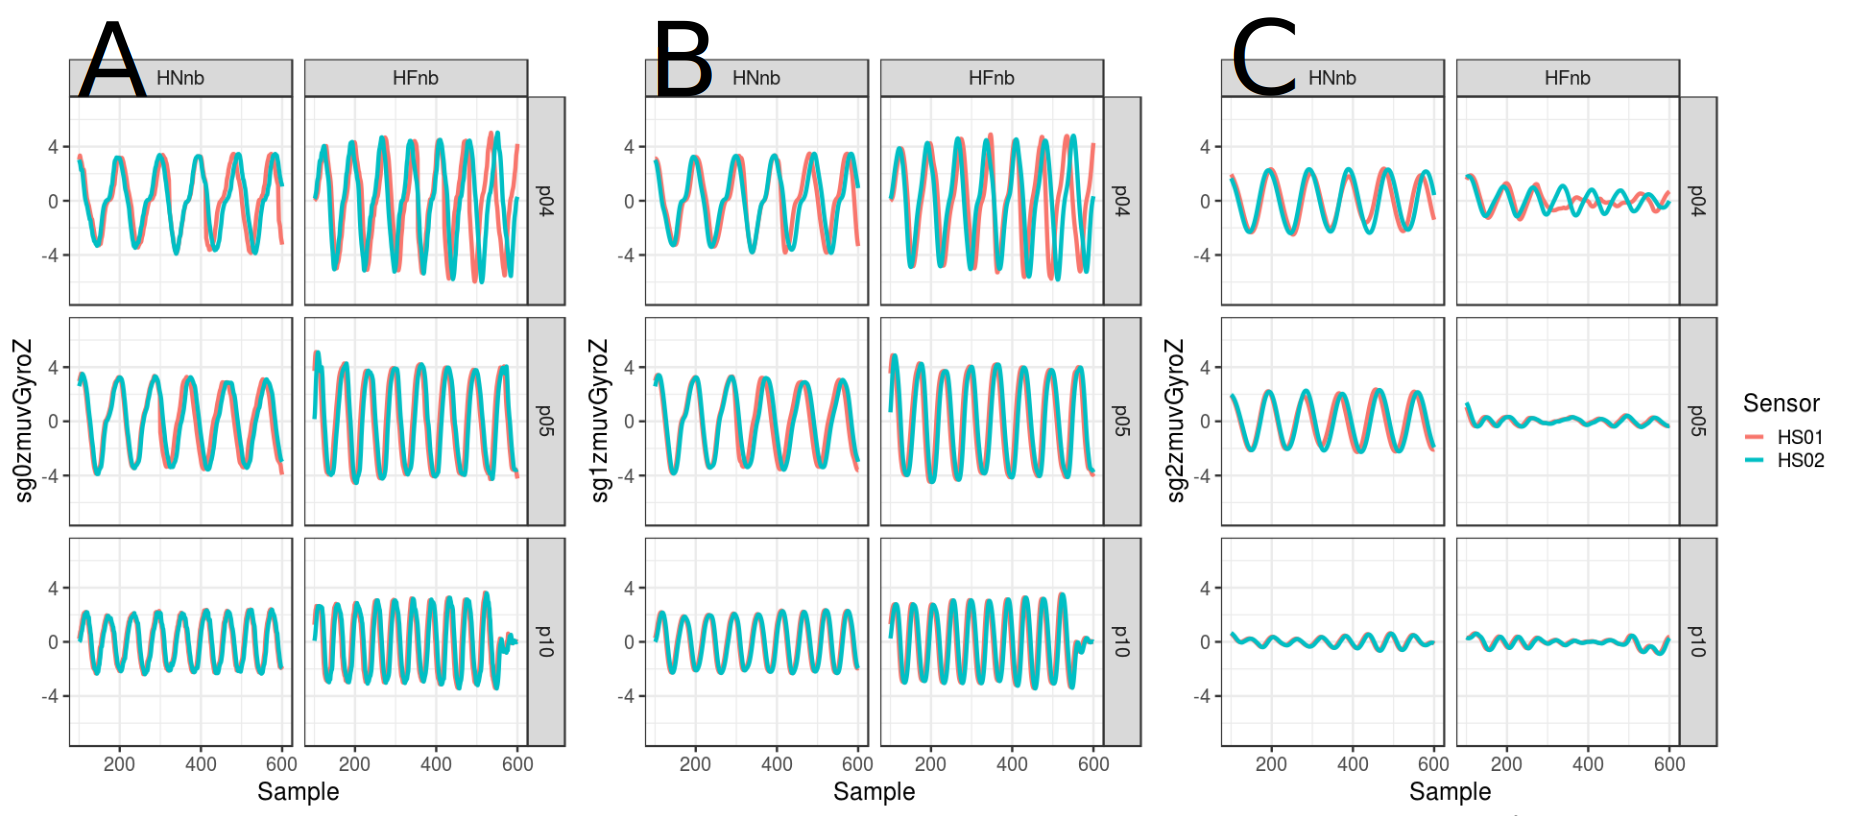
\includegraphics[width=1.0\textwidth]{tsHnb}
    	\caption{ 
	{\bf Time series for horizontal arm movements (no beat).}
		(A) raw-normalised (sg0zmuvGyroZ), 
		(B) normalised-smoothed 1 (sg1zmuvGyroZ) and
		(C) normalised-smoothed 2 (sg2zmuvGyroZ).
		Time series are for only three participants (p04, p05, and p10) 
		for horizontal movements in normal and faster velocity with
		no beat	(HNnb, HFnb) using the normalised 
		GyroZ axis (zmuvGyroZ) and two sensors attached to 
		the participant wrist (HS01, HS02).
	R code to reproduce the figure is available from \cite{hwum2018}.
        }
    \label{fig:tsHnb}
\end{figure}
%%---------------------------------(FIGURE)-----------------------------------
%%---------------------------------(FIGURE)------------------------------------
\begin{figure}[!h]
\centering
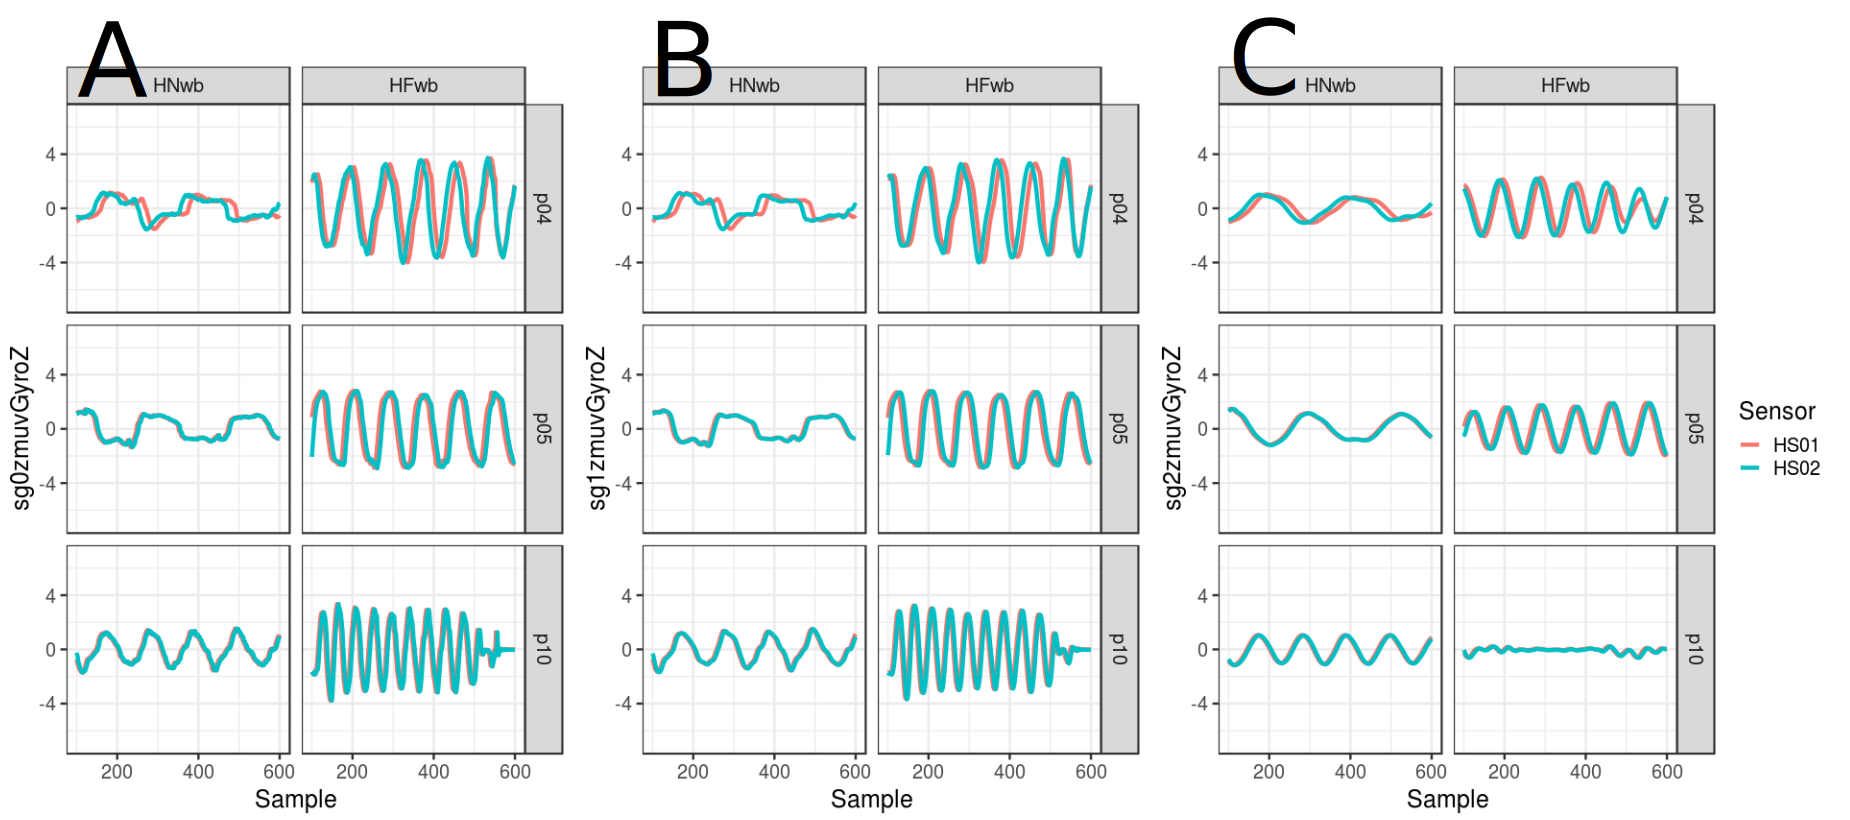
\includegraphics[width=1.0\textwidth]{tsHwb}
    	\caption{ 
	{\bf Time series for horizontal arm movements (with beat).}
		(A) raw-normalised (sg0zmuvGyroZ), 
		(B) normalised-smoothed 1 (sg1zmuvGyroZ) and
		(C) normalised-smoothed 2 (sg2zmuvGyroZ).
		Time series are for only three participants (p04, p05, and p10) 
		for horizontal movements in normal and faster velocity with
		beat (HNwb, HFwb) using the normalised 
		GyroZ axis (zmuvGyroZ) and two sensors attached to 
		the participant wrist (HS01, HS02).
	R code to reproduce the figure is available from \cite{hwum2018}.
        }
    \label{fig:tsHwb}
\end{figure}
%%---------------------------------(FIGURE)------------------------------------
%%---------------------------------(FIGURE)-------------------------------------
\begin{figure}[!h]
\centering
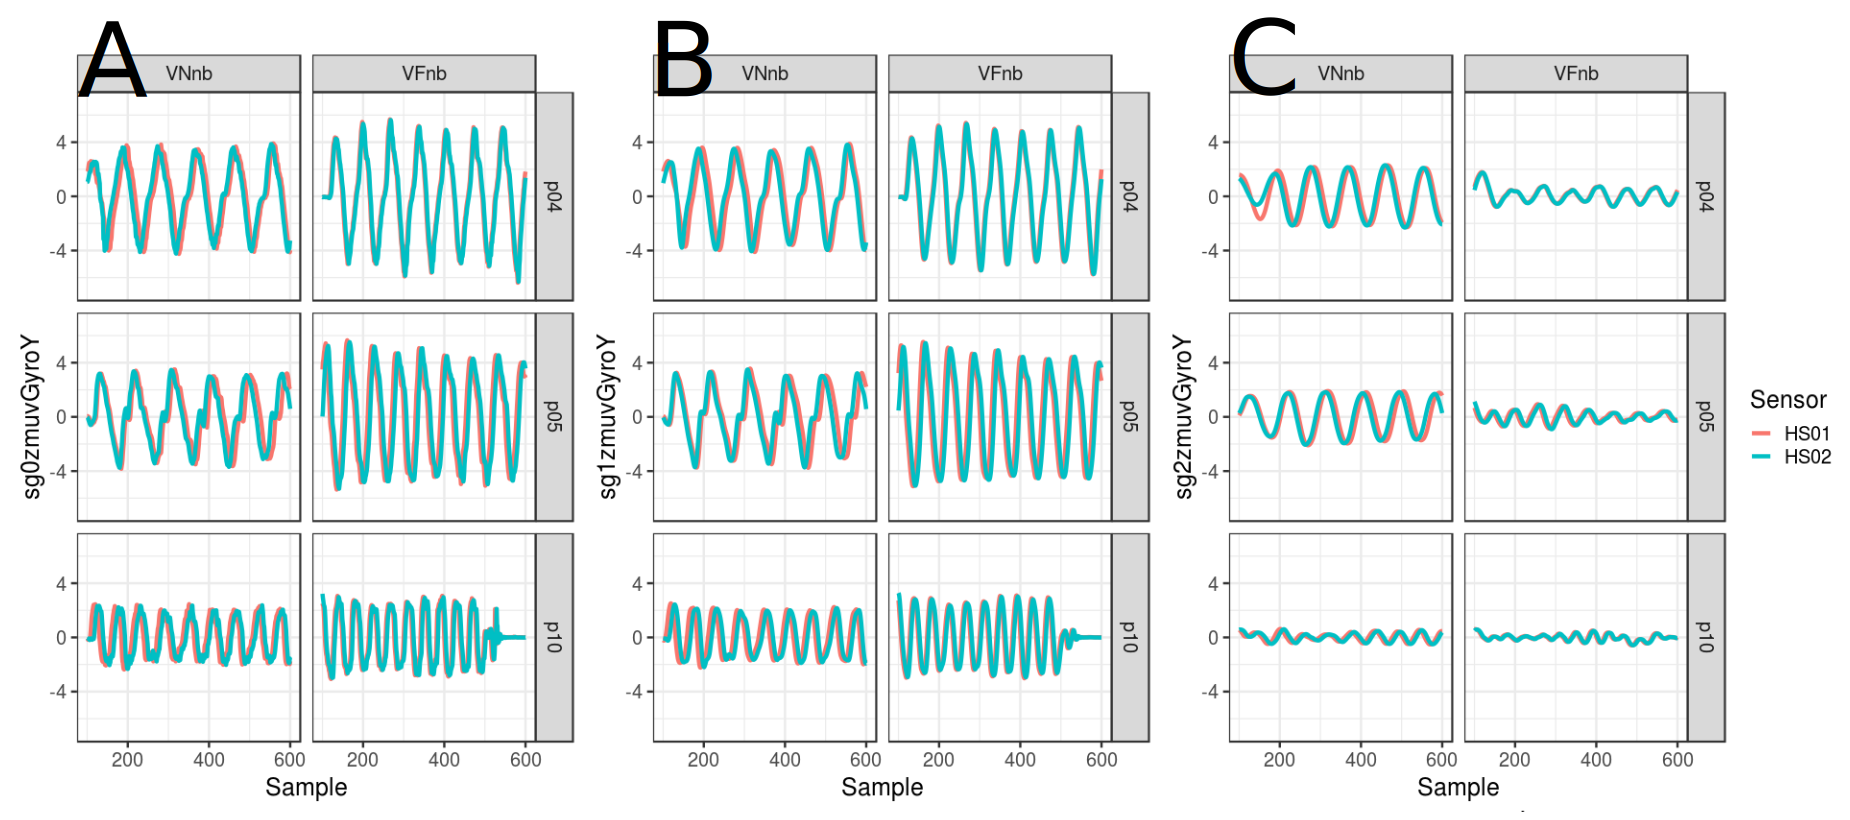
\includegraphics[width=1.0\textwidth]{tsVnb}
    	\caption{ 
	{\bf Time series for vertical arm movements (no beat).}
		(A) raw-normalised (sg0zmuvGyroY), 
		(B) normalised-smoothed 1 (sg1zmuvGyroY) and
		(C) normalised-smoothed 2 (sg2zmuvGyroY).
		Time series are for only three participants (p04, p05, and p10) 
		for vertical movements in normal and faster velocity with
		no beat	(VNnb, VFnb) using the normalised 
		GyroY axis (zmuvGyroY) and two sensors attached to 
		the participant wrist (HS01, HS02).
	R code to reproduce the figure is available from \cite{hwum2018}.
        }
    \label{fig:tsVnb}
\end{figure}
%%---------------------------------(FIGURE)------------------------------------
%%---------------------------------(FIGURE)-------------------------------------
\begin{figure}[!h]
\centering
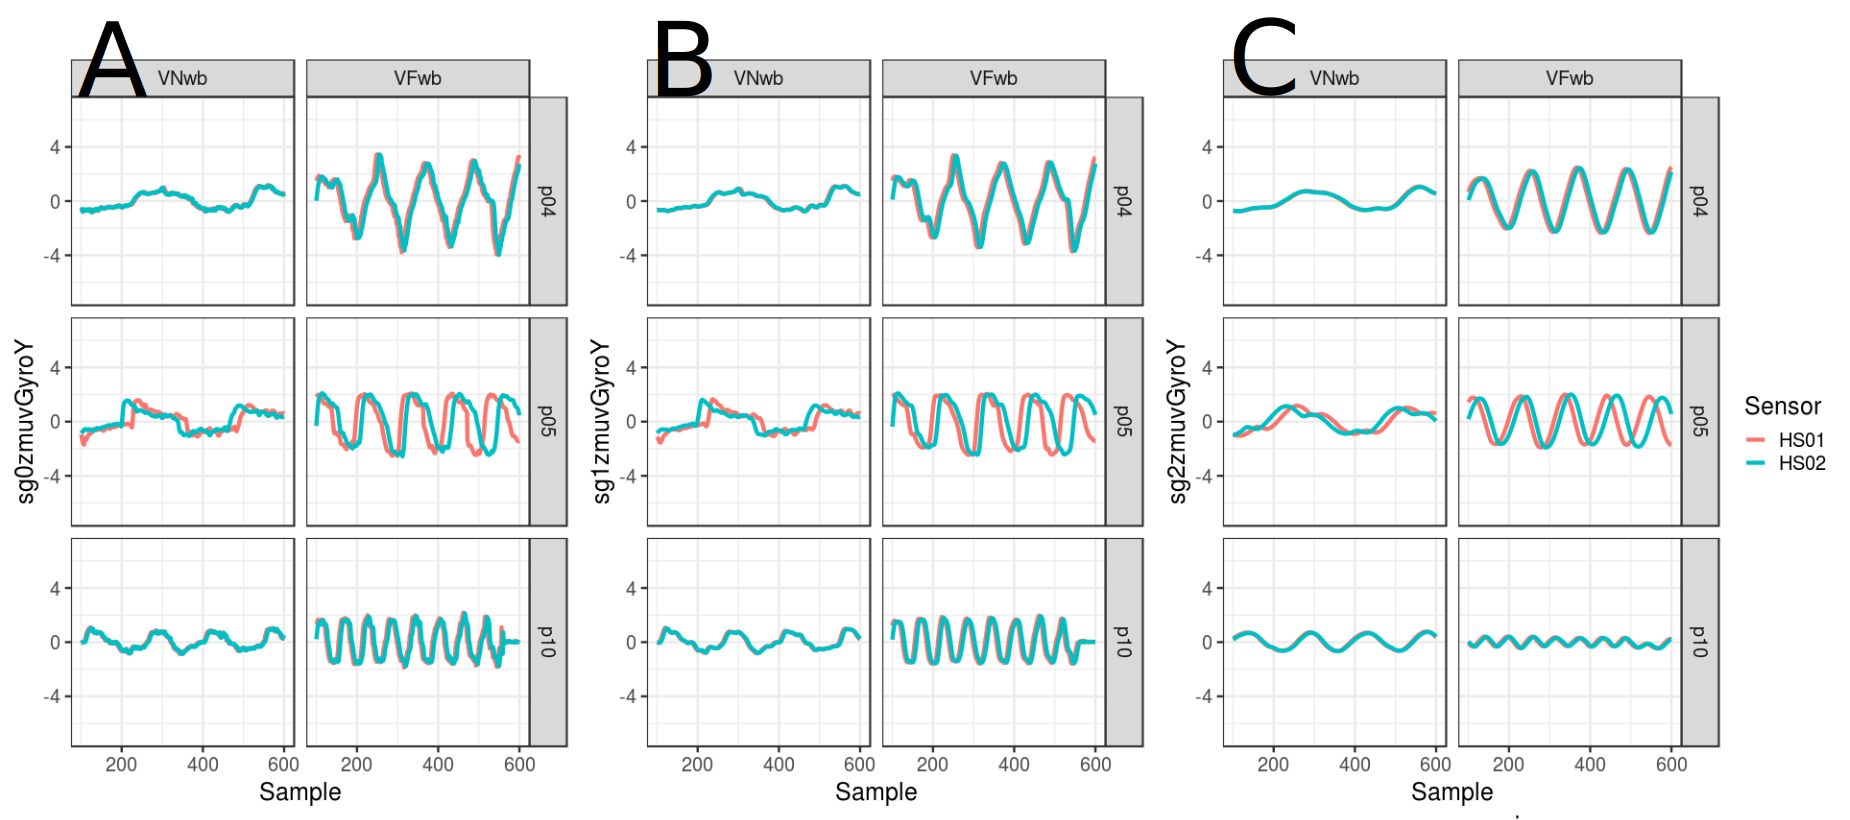
\includegraphics[width=1.0\textwidth]{tsVwb}
    	\caption{ 
	{\bf Time series for vertical arm movements (with beat).}
		(A) raw-normalised (sg0zmuvGyroY), 
		(B) normalised-smoothed 1 (sg1zmuvGyroY) and
		(C) normalised-smoothed 2 (sg2zmuvGyroY).
		Time series are for only three participants (p04, p05, and p10) 
		for vertical movements in normal and faster velocity with
		beat (VNwb, VFwb) using the normalised 
		GyroY axis (zmuvGyroY) and two sensors attached to 
		the participant wrist (HS01, HS02).
	R code to reproduce the figure is available from \cite{hwum2018}.
        }
    \label{fig:tsVwb}
\end{figure}
%%---------------------------------(FIGURE)------------------------------------





\section{Minimum Embedding Parameters}

\subsection{Minimum dimension embedding values}
Values of minimum embedding dimensions for horizontal normal arm movements 
with no beat (HNnb) and horizontal faster arm movements 
with no beat (HFnb) are shown in Fig \ref{fig:caoHnb} which values of 
minimum embedding dimensions present a fluctuation of values between four 
and seven over six participants.
It can also be noted a slightly variation of minimum embedding dimension values 
over participants when comparing HS01 and HS02 (Fig \ref{fig:caoHnb}(A, B)).
With regards to the smoothness of the time series,
the minimum embedding values are also smoothed showing less variations of
values over six participants (Fig \ref{fig:caoHnb}).

Values of minimum embedding dimension for horizontal normal arm movements 
with beat (HNwb) and horizontal faster arm movements with beat (HFwb) 
are shown in Fig \ref{fig:caoHwb} where is shown a fluctuations of values
for minimum embedding dimension between five and seven.
Similarly as in Fig \ref{fig:caoHnb}, Fig \ref{fig:caoHwb} show changes of 
minimum embedding dimension between participants and the smoothness of the 
time series also affects the smoothness of minimum embedding dimension values.
%%---------------------------------(FIGURE)-------------------------------------
\begin{figure}[!h]
\centering
\includegraphics[width=1.0\textwidth]{cao_Hnb_w10}
	\caption{
	{\bf Minimum embedding dimensions for horizontal arm movements 
	(no beat).} 
		(A, B) Horizontal Normal with no beat (HNnb), and 
		(C, D) Horizontal Faster with no beat (HFnb) movements.
		(A, C) Sensor 01 attached to the participant (HS01), and
		(B, D) sensor 02 attached to the participant (HS02).
		Minimum embedding dimensions are for six participants 
		(p01, p04, p05, p10, p11, p15) with three smoothed signals 
		(sg0zmuvGyroZ, sg1zmuvGyroZ and sg2zmuvGyroZ)
		and window lenght of 10-sec (500 samples).
		R code to reproduce the figure is available 
		from \cite{hwum2018}.
        }
    \label{fig:caoHnb}
\end{figure}
%%---------------------------------(FIGURE)-------------------------------------
%%---------------------------------(FIGURE)-------------------------------------
\begin{figure}[!h]
\centering
\includegraphics[width=1.0\textwidth]{cao_Hwb_w10}
	\caption{
	{\bf Minimum embedding dimensions for horizontal arm movements 
	(with beat).} 
		(A, B) Horizontal Normal with beat (HNwb), and
		(C, D) Horizontal Faster with beat (HFwb) movements.
		(A, C) Sensor 01 attached to the participant (HS01), and
		(B, D) sensor 02 attached to the participant (HS02).
		Minimum embedding dimensions are for six participants 
		(p01, p04, p05, p10, p11, p15) with three smoothed signals 
		(sg0zmuvGyroZ, sg1zmuvGyroZ and sg2zmuvGyroZ)
		and window lenght of 10-sec (500 samples).
		R code to reproduce the figure is available 
		from \cite{hwum2018}.
        }
    \label{fig:caoHwb}
\end{figure}
%%---------------------------------(FIGURE)-------------------------------------


Values of minimum embedding dimension for vertical arm movements with no beat
are shown in Figs \ref{fig:caoVnb}(A, B) where the smoothness 
of the time series have little effect on the minimum embedding dimension 
values, whereas smoothness of time series affects the smoothness of the 
minimum embedding values for vertical faster arm movements with no beats 
(Fig \ref{fig:caoVnb}(C, D)).

Fig \ref{fig:caoVwb} shows the variation of minimum embedding values for 
vertical arm movements with beat where the smoothness of the time series
affects both vertical normal and vertical faster movements with a slight 
decrease on each of the values as the smoothness increase.
%%---------------------------------(FIGURE)-------------------------------------
\begin{figure}[!h]
\centering
\includegraphics[width=1.0\textwidth]{cao_Vnb_w10}
	\caption{
	{\bf Minimum embedding dimensions for vertical arm movements 
	(no beat).} 
		(A, B) Vertical Normal with no beat (VNnb), and 
		(C, D) Vertical Faster with no beat (VFnb) movements.
		(A, C) Sensor 01 attached to the participant (HS01), and
		(B, D) sensor 02 attached to the participant (HS02).
		Minimum embedding dimensions are for six participants 
		(p01, p04, p05, p10, p11, p15) with three smoothed signals 
		(sg0zmuvGyroZ, sg1zmuvGyroZ and sg2zmuvGyroZ)
		and window lenght of 10-sec (500 samples).
		R code to reproduce the figure is available 
		from \cite{hwum2018}.
        }
    \label{fig:caoVnb}
\end{figure}
%%---------------------------------(FIGURE)-------------------------------------
%%---------------------------------(FIGURE)-------------------------------------
\begin{figure}[!h]
\centering
\includegraphics[width=1.0\textwidth]{cao_Vwb_w10}
	\caption{
	{\bf Minimum embedding dimensions for vertical arm movements 
	(with beat).} 
		(A, B) Vertical Normal with beat (VNwb), and
		(C, D) Vertical Faster with beat (VFwb) movements.
		(A, C) Sensor 01 attached to the participant (HS01), and
		(B, D) sensor 02 attached to the participant (HS02).
		Minimum embedding dimensions are for six participants 
		(p01, p04, p05, p10, p11, p15) with three smoothed signals 
		(sg0zmuvGyroZ, sg1zmuvGyroZ and sg2zmuvGyroZ)
		and window lenght of 10-sec (500 samples).
		R code to reproduce the figure is available 
		from \cite{hwum2018}.
        }
    \label{fig:caoVwb}
\end{figure}
%%---------------------------------(FIGURE)-------------------------------------




\subsection{Minimum delay embedding values}
The general behavior for horizontal and vertical arm movements with regards
to the smoothness of the time series is that the first minimum AMI values 
increase as the increase of the smoothness which is due to smoothed AMI 
curves 
(Figs \ref{fig:amiHnb}, \ref{fig:amiHwb}, \ref{fig:amiVnb} and 
\ref{fig:amiVwb}).

Fluctuations of minimum AMI values from sensor HS01 are more evident than 
for sensor HS02 for horizontal normal arm movements with no beat 
(Fig \ref{fig:amiHnb}(A, B)),
whereas fluctuations of minimum AMI values from sensors HS01 and HS02 
for horizontal faster arm movements with no beat appear to be similar 
(Fig \ref{fig:amiHnb}(C, D)).
Similarly, fluctuations of minimum AMI values are more evidently for 
horizontal normal arm movements with beat (Fig \ref{fig:amiHwb}(A, B)) than 
horizontal faster arm movements with beat (Fig \ref{fig:amiHwb}(C, D)).

As smoothness increase, minimum AMI values for vertical normal arm movements 
with no beat appear to fluctuate more (Figs \ref{fig:amiVnb}(A, B))
than vertical faster arm movements with no beat (Figs \ref{fig:amiVnb}(C, D)),
whereas for vertical normal and vertical faster arm movements with beat 
the fluctuation of minimum AMI values is more evidently,
specially when comparing vertical normal arm movements 
(Figs \ref{fig:amiVwb}(A, B)) with vertical faster arm movements 
(Figs \ref{fig:amiVwb}(C, D)).

%%---------------------------------(FIGURE)-------------------------------------
\begin{figure}[!h]
\centering
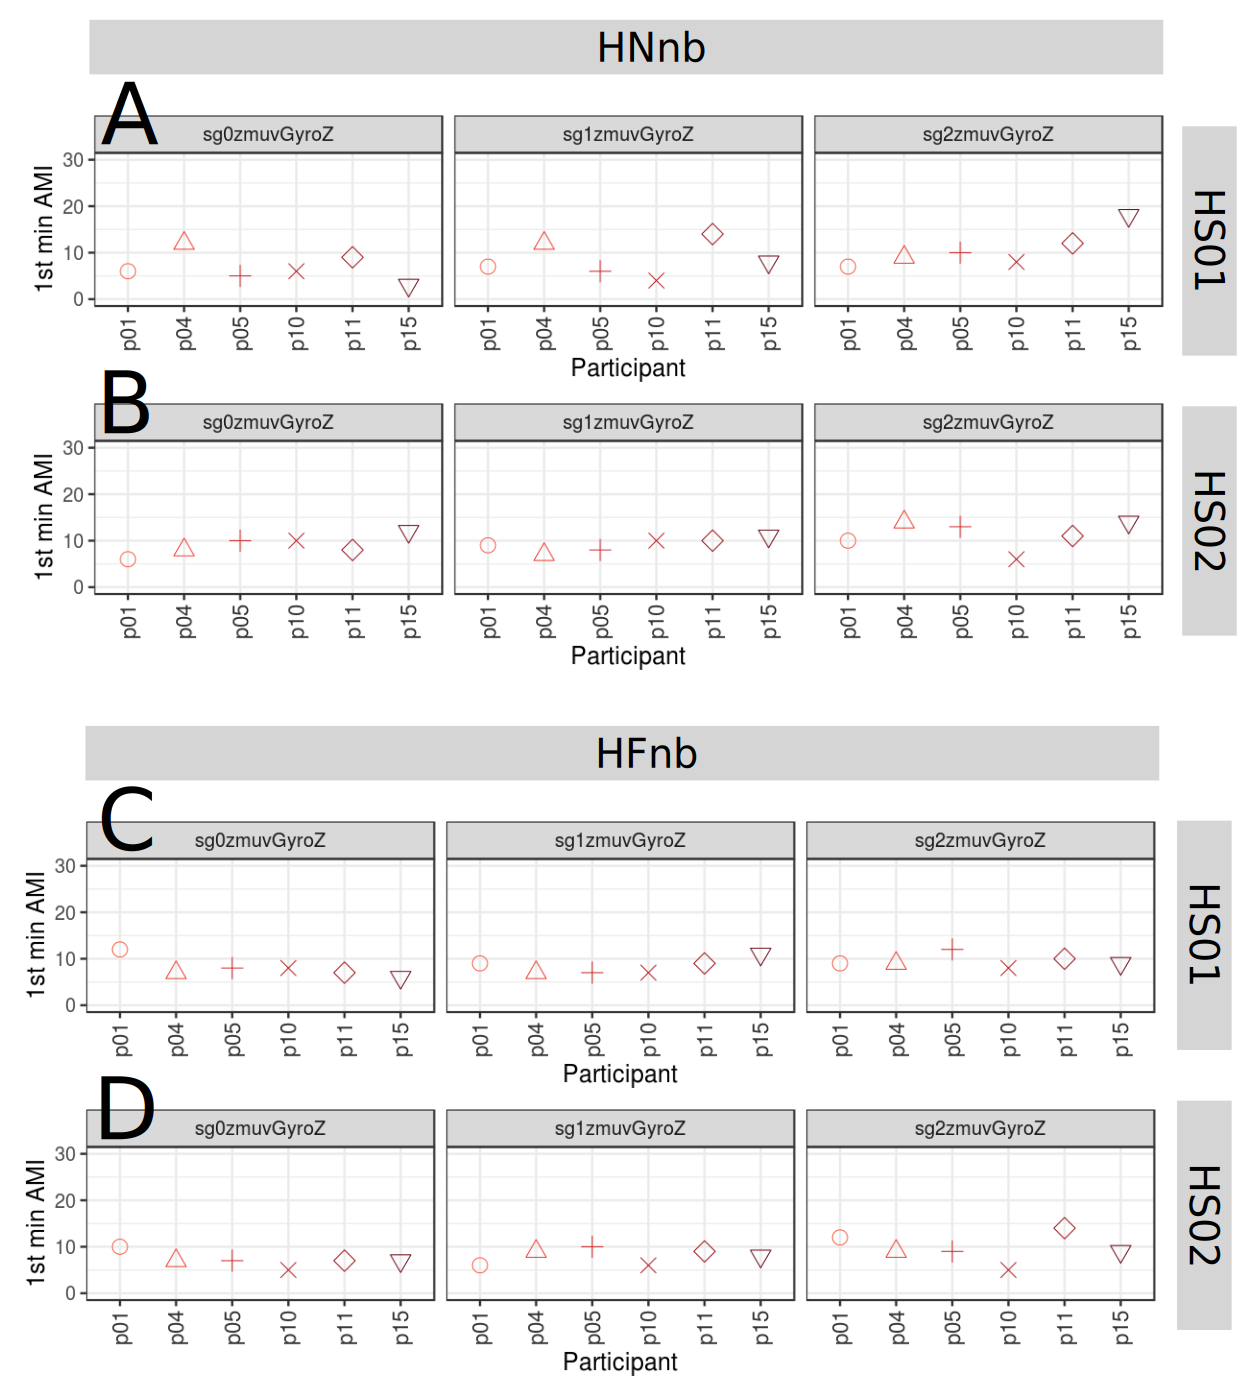
\includegraphics[width=1.0\textwidth]{ami_Hnb_w10}
	\caption{
	{\bf First minimum AMI values for horizontal arm movements (no beat).}
		(A, B) Horizontal Normal with no beat (HNnb), and 
		(C, D) Horizontal Faster with no beat (HFnb) movements.
		(A, C) Sensor attached to the participant (HS01), and
		(B, D) sensor attached to the participant (HS02).
		First minimum AMI values are for six participants 
		(p01, p04, p05, p10, p11, p15) with three smoothed 
		signals (sg0zmuvGyroZ, sg1zmuvGyroZ and sg2zmuvGyroZ) and 
		window lenght of 10-sec (500 samples).
		R code to reproduce the figure is available 
		from \cite{hwum2018}.
        }
    \label{fig:amiHnb}
\end{figure}
%%---------------------------------(FIGURE)------------------------------------
%%---------------------------------(FIGURE)-------------------------------------
\begin{figure}[!h]
\centering
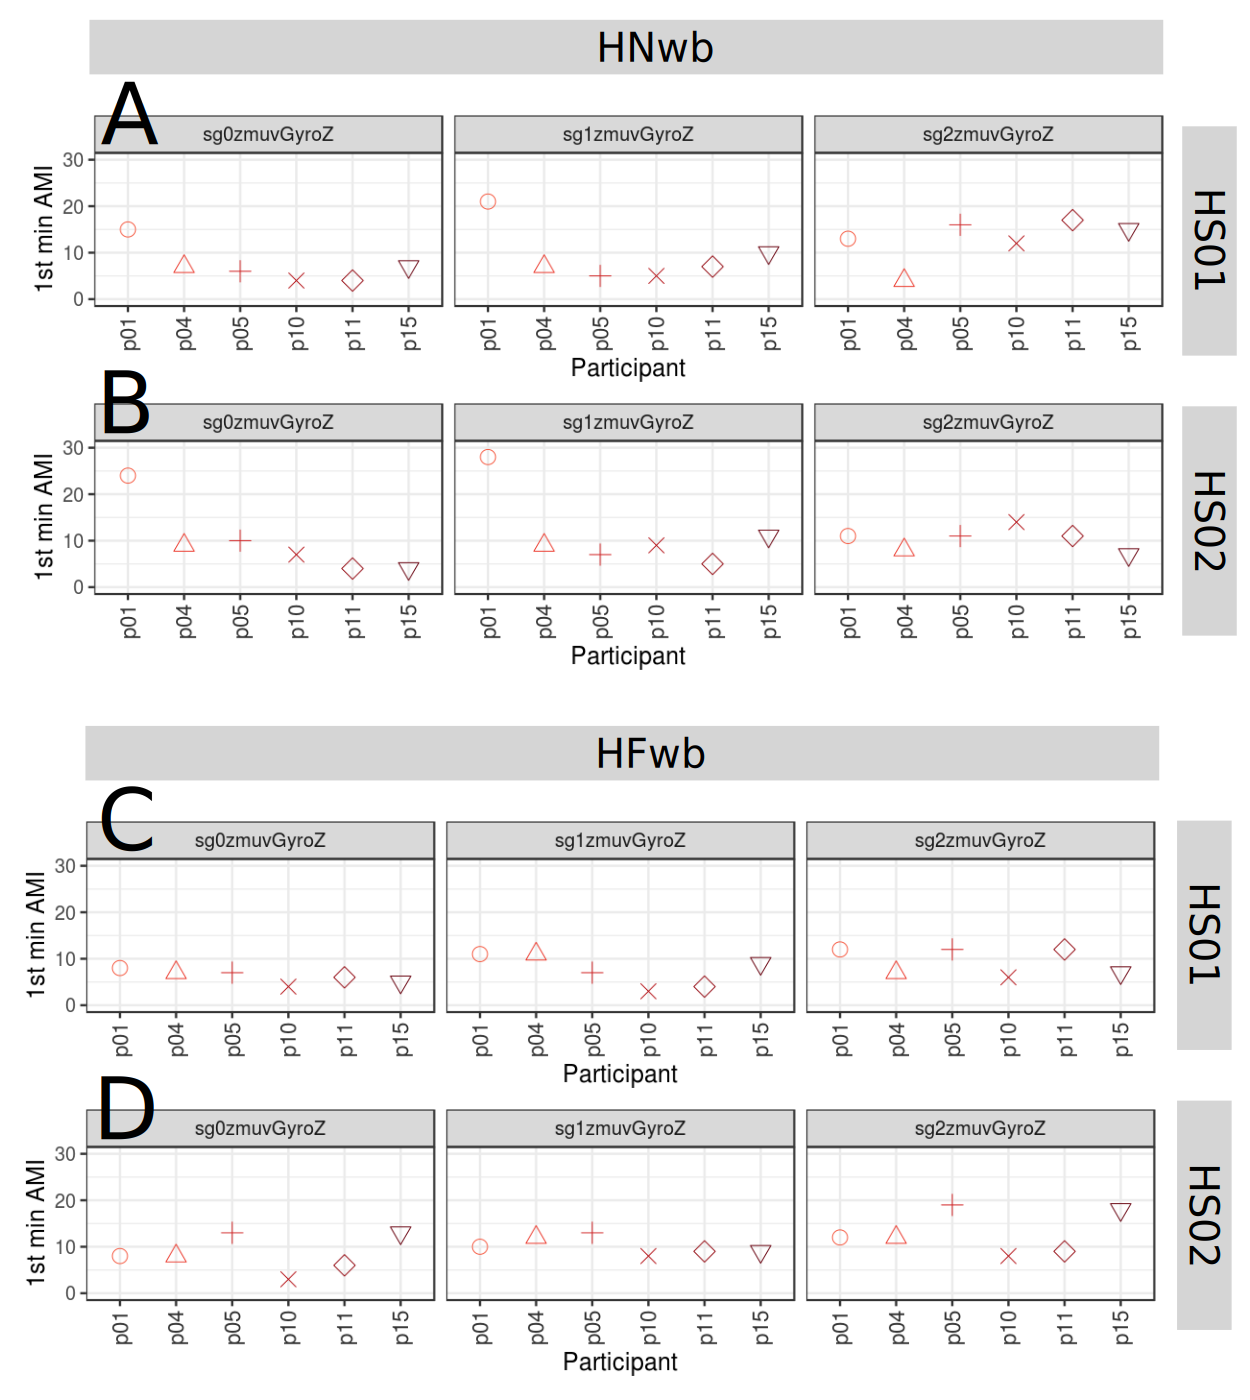
\includegraphics[width=1.0\textwidth]{ami_Hwb_w10}
	\caption{
	{\bf First minimum AMI values for horizontal arm movements (with beat).}
		(A, B) Horizontal Normal with beat (HNwb), and 
		(C, D) Horizontal Faster with beat (HFwb) movements.
		(A, C) Sensor attached to the participant (HS01), and
		(B, D) sensor attached to the participant (HS02).
		First minimum AMI values are for six participants 
		(p01, p04, p05, p10, p11, p15) with three smoothed 
		signals (sg0zmuvGyroZ, sg1zmuvGyroZ and sg2zmuvGyroZ) and 
		window lenght of 10-sec (500 samples).
		R code to reproduce the figure is available 
		from \cite{hwum2018}.
        }
    \label{fig:amiHwb}
\end{figure}
%%---------------------------------(FIGURE)------------------------------------

%%---------------------------------(FIGURE)------------------------------------
\begin{figure}[!h]
\centering
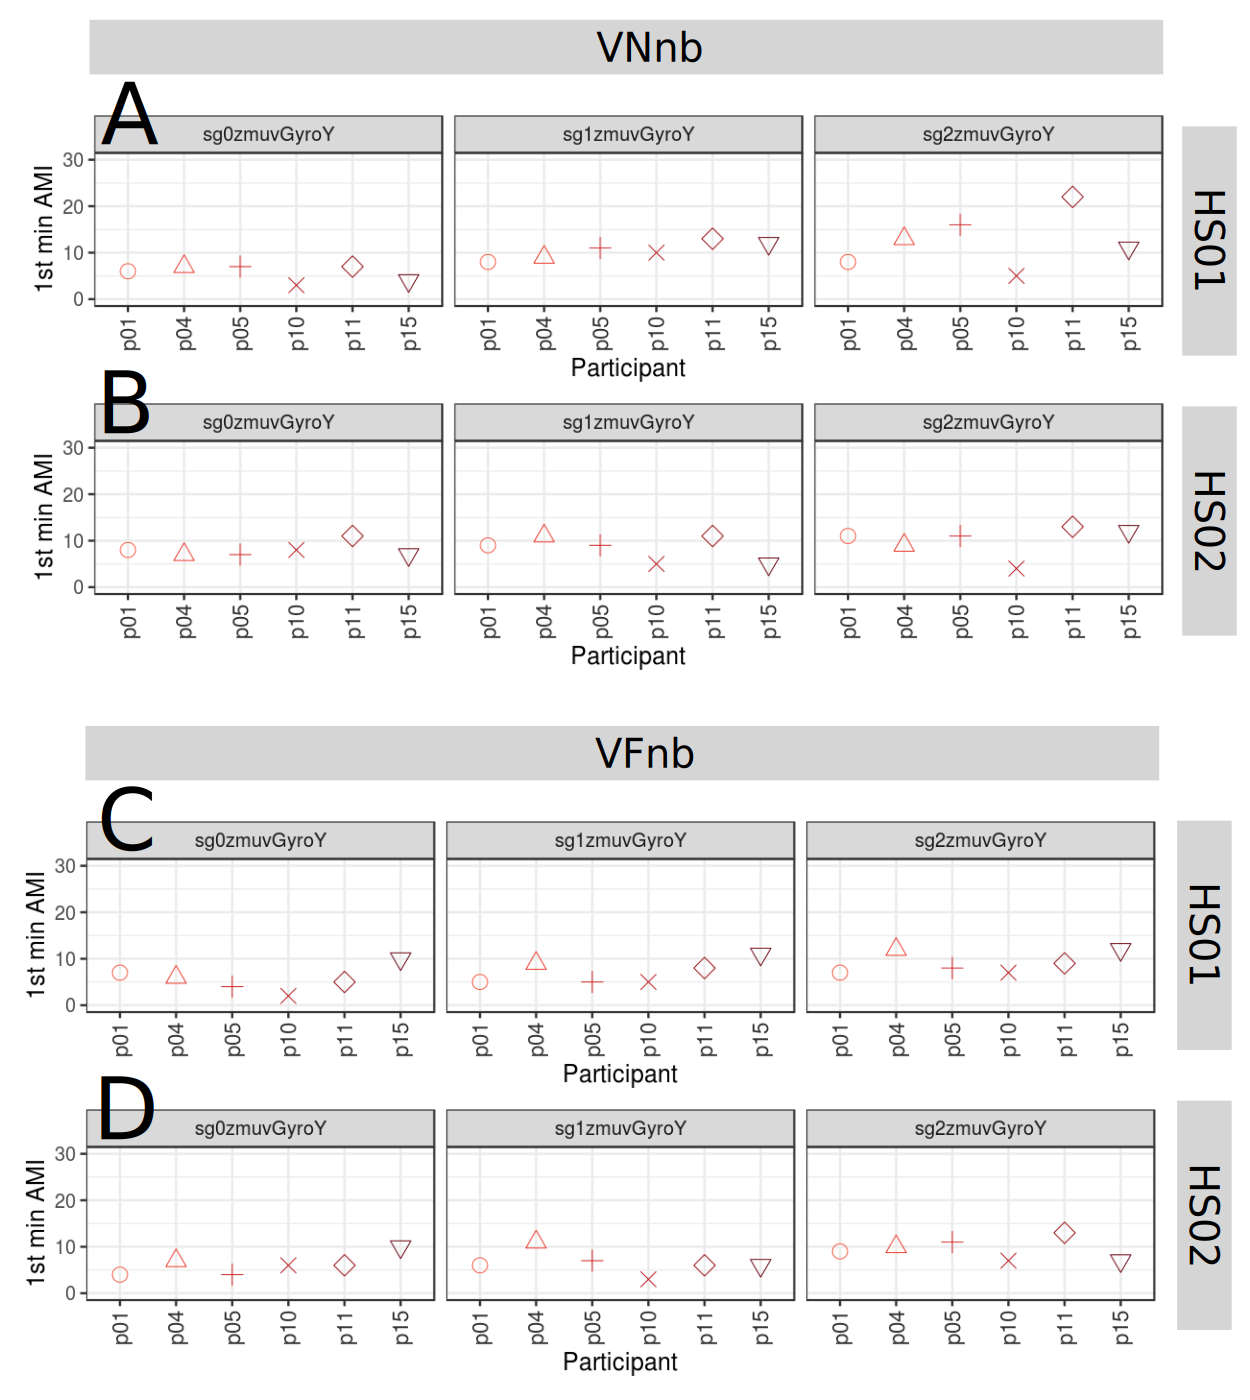
\includegraphics[width=1.0\textwidth]{ami_Vnb_w10}
	\caption{
	{\bf First minimum AMI values for vertical arm movements (no beat).}
		(A, B) Vertical Normal with no beat (VNnb), and 
		(C, D) Vertical Faster with no beat (VFnb) movements.
		(A, C) Sensor attached to the participant (HS01), and
		(B, D) sensor attached to the participant (HS02).
		First minimum AMI values are for six participants 
		(p01, p04, p05, p10, p11, p15) with three smoothed 
		signals (sg0zmuvGyroZ, sg1zmuvGyroZ and sg2zmuvGyroZ) and 
		window lenght of 10-sec (500 samples).
		R code to reproduce the figure is available 
		from \cite{hwum2018}.
        }
    \label{fig:amiVnb}
\end{figure}
%%---------------------------------(FIGURE)------------------------------------

%%---------------------------------(FIGURE)------------------------------------
\begin{figure}[!h]
\centering
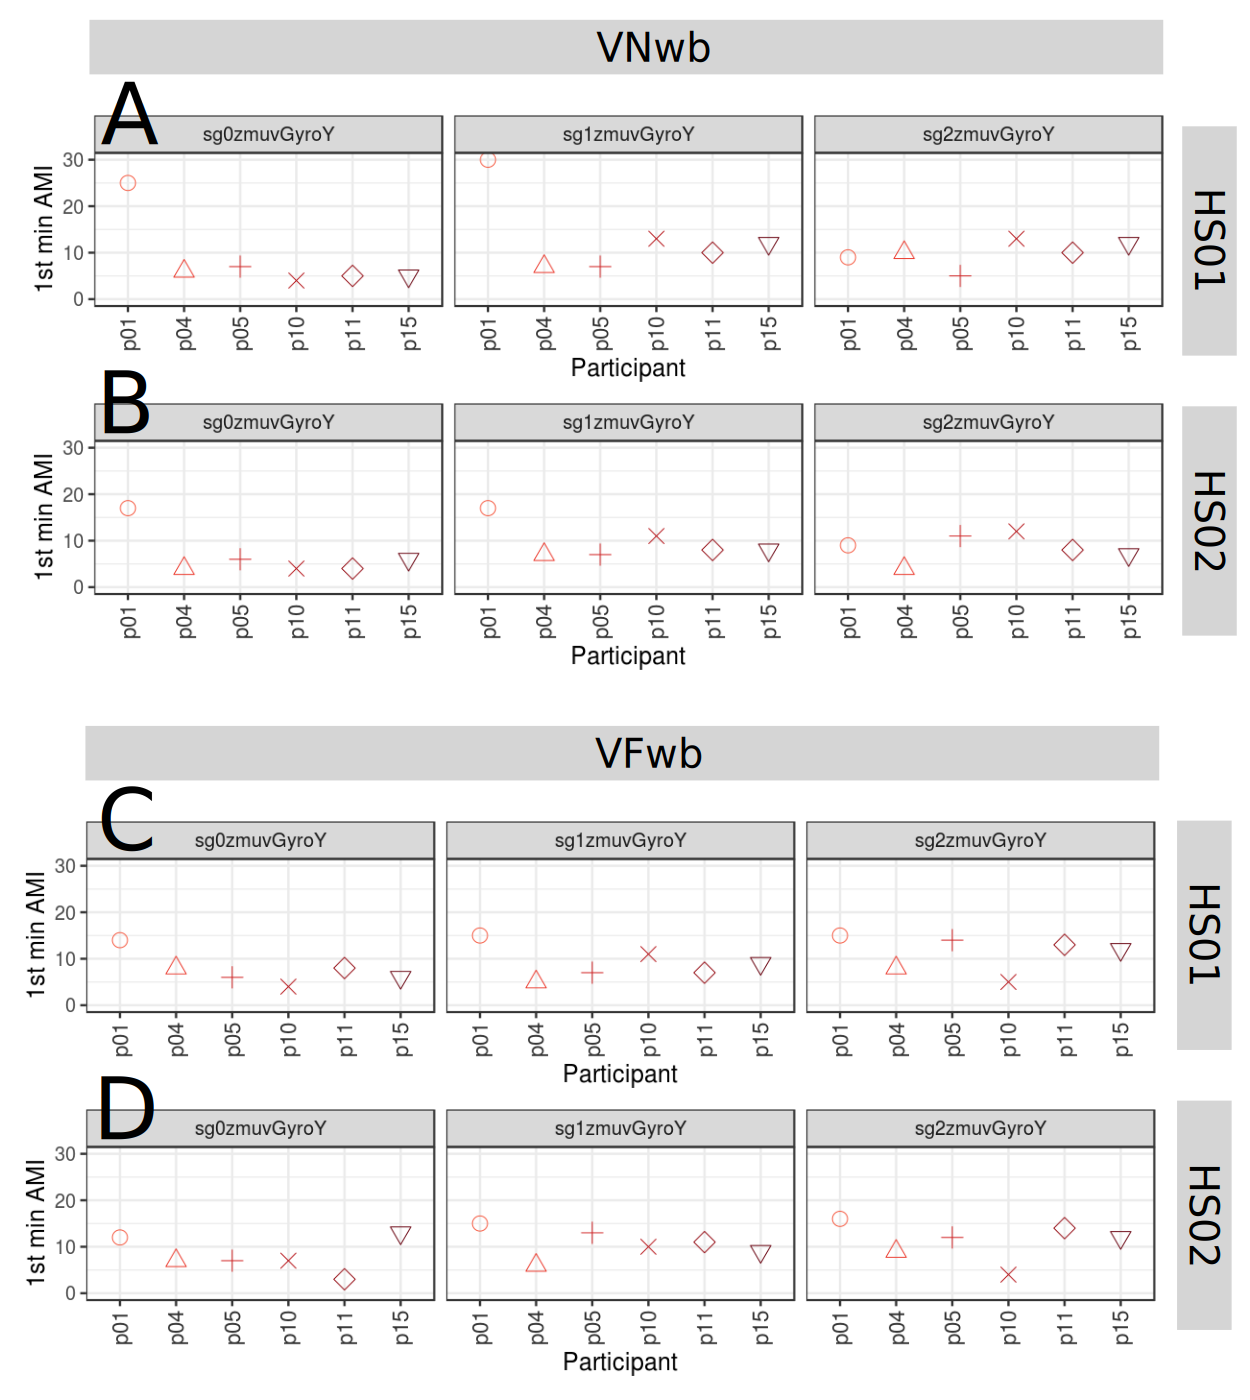
\includegraphics[width=1.0\textwidth]{ami_Vwb_w10}
	\caption{
	{\bf First minimum AMI values for vertical arm movements (with beat).}
		(A, B) Vertical Normal with beat (VNwb), and 
		(C, D) Vertical Faster with beat (VFwb) movements.
		(A, C) Sensor attached to the participant (HS01), and
		(B, D) sensor attached to the participant (HS02).
		First minimum AMI values are for six participants 
		(p01, p04, p05, p10, p11, p15) with three smoothed 
		signals (sg0zmuvGyroZ, sg1zmuvGyroZ and sg2zmuvGyroZ) and 
		window lenght of 10-sec (500 samples).
		R code to reproduce the figure is available 
		from \cite{hwum2018}.
        }
    \label{fig:amiVwb}
\end{figure}
%%---------------------------------(FIGURE)------------------------------------



\subsection{Average minimum embedding parameters}
The average minimum embedding parameters is computed with 
a sample mean of $\overline{m}_0=9$ from the minimum values 
of $E_{1}(m)$ of Figs \ref{fig:caoHnb}, \ref{fig:caoHwb}, 
\ref{fig:caoVnb}, and \ref{fig:caoVwb} 
and a sample mean of $\overline{\tau}_0=6$ from minimum values of AMIs 
of Figs \ref{fig:amiHnb}, \ref{fig:amiHwb}, 
\ref{fig:amiVnb}, and \ref{fig:amiVwb} (Section \ref{sec:overall_minMT}).
Hence, Reconstructed State Spaces (RSSs), Recurrence Plots (RPs), and
Recurrence Quantification Analysis (RQA) metrics
are computed with the average minimum embedding parameters 
($\overline{m_0}=9$, $\overline{\tau_0}=6$).


\section{Reconstructed state spaces with UTDE}
Reconstructed state spaces for horizontal normal and horizontal faster 
arm movements with no beat are shown in Fig \ref{fig:rss_Hnb_w500}.
The smoothness of the time series show a slightly change of smoothed 
trajectories in the RSSs for sg0zmuvGyroZ and sg1zmuvGyroZ, while the 
RSSs trajectories for sg2zmuvGyroZ appear to be distorted 
(Fig \ref{fig:rss_Hnb_w500}).
One can see slightly differences in the RSSs trajectories when comparing 
sensors HS01 and HS02 for horizontal normal arm movement with no beat 
(Fig \ref{fig:rss_Hnb_w500}(A, B)) and horizontal faster arm movements 
with no beat (Fig \ref{fig:rss_Hnb_w500}(C, D)).
With regards to the type of movement, the RSSs trajectories appear 
to change little when comparing horizontal normal with faster arm movements 
(Fig \ref{fig:rss_Hnb_w500}).

Fig \ref{fig:rss_Hwb_w500} shows trajectories of the reconstructed 
state space for horizontal normal and horizontal faster arm movements 
while beat sounds. Hence, as in Fig \ref{fig:rss_Hnb_w500}, 
it can also be noted in Fig \ref{fig:rss_Hwb_w500} that the smoothness 
of sg0zmuvGyroZ and sg1zmuvGyroZ appear to affect little the RSSs 
trajectories, while RSSs trajectories for sg2zmuvGyroZ substantially change 
so as to show different patterns. However, the trajectories in the RSS 
appear to change little when comparing the differences between the type 
of sensors HS01 and HS02 (Fig \ref{fig:rss_Hwb_w500}).
For the type of movements, trajectories show differences for horizontal
normal and horizontal faster arm movements (Fig \ref{fig:rss_Hwb_w500}).

Fig \ref{fig:rss_Vnb_w500} show trajectories for reconstructed state spaces
of vertical normal and vertical faster arm movements with no beat. 
Smoothness of the RSSs trajectories is slightly noticed for sg0zmuvGyroY and
sg1zmuvGyroY, whereas RSSs trajectories for sg2zmuvGyroY are evidently 
different (Fig \ref{fig:rss_Vnb_w500}).
When comparing the RSSs trajectories from sensors HS01 and HS02,
it can be noted little change, whereas the comparison from type of movement, 
the trajectories difference is more notable (Fig \ref{fig:rss_Vnb_w500}).

Fig \ref{fig:rss_Vwb_w500} show trajectories for reconstructed state space
of vertical normal and vertical faster arm movements for participants 
hearing a beat. Smoothness of RSSs trajectories appear to show slightly 
differences between sg0zmuvGyroY and sg1zmuvGyroY, however RSSs trajectories 
for sg2zmuvGyroY are different (Fig \ref{fig:rss_Vwb_w500}).
With regards to the type of sensor HS01 and HS02, RSSs trajectories appear 
to change little, whereas for type of activity of normal and faster arm 
movements, RSSs trajectories show evidently differences 
(Fig \ref{fig:rss_Vwb_w500}).


%%---------------------------------(FIGURE)-------------------------------------
\begin{figure}[!h]
\centering
\includegraphics[height=0.8\textheight]{rss_Hnb_w500}
\caption{
	{\bf RSSs for horizontal arm movements (no beat).}
	Reconstructed state spaces of participant p01 for 
	(A, B) horizontal normal movements with no beat (HNnb) and 
	(C, D) horizontal faster velocity with no beat (HFnb).
	Time series for raw-normalised (sg0zmuvGyroZ), 
	normalised-smoothed 1 (sg1zmuvGyroZ) and 
	normalised-smoothed 2 (sg2zmuvGyroZ) with
	(A, C) sensor attached to the participant (HS01), and
	(B, D) sensor attached to the participant (HS02).	
	Reconstructed state spaces were computed with 
	embedding parameters $m=9$, $\tau=6$.
	R code to reproduce the figure is available from \cite{hwum2018}.
        }
     \label{fig:rss_Hnb_w500}
\end{figure}
%%---------------------------------(FIGURE)------------------------------------



%%---------------------------------(FIGURE)-------------------------------------
\begin{figure}[!h]
\centering
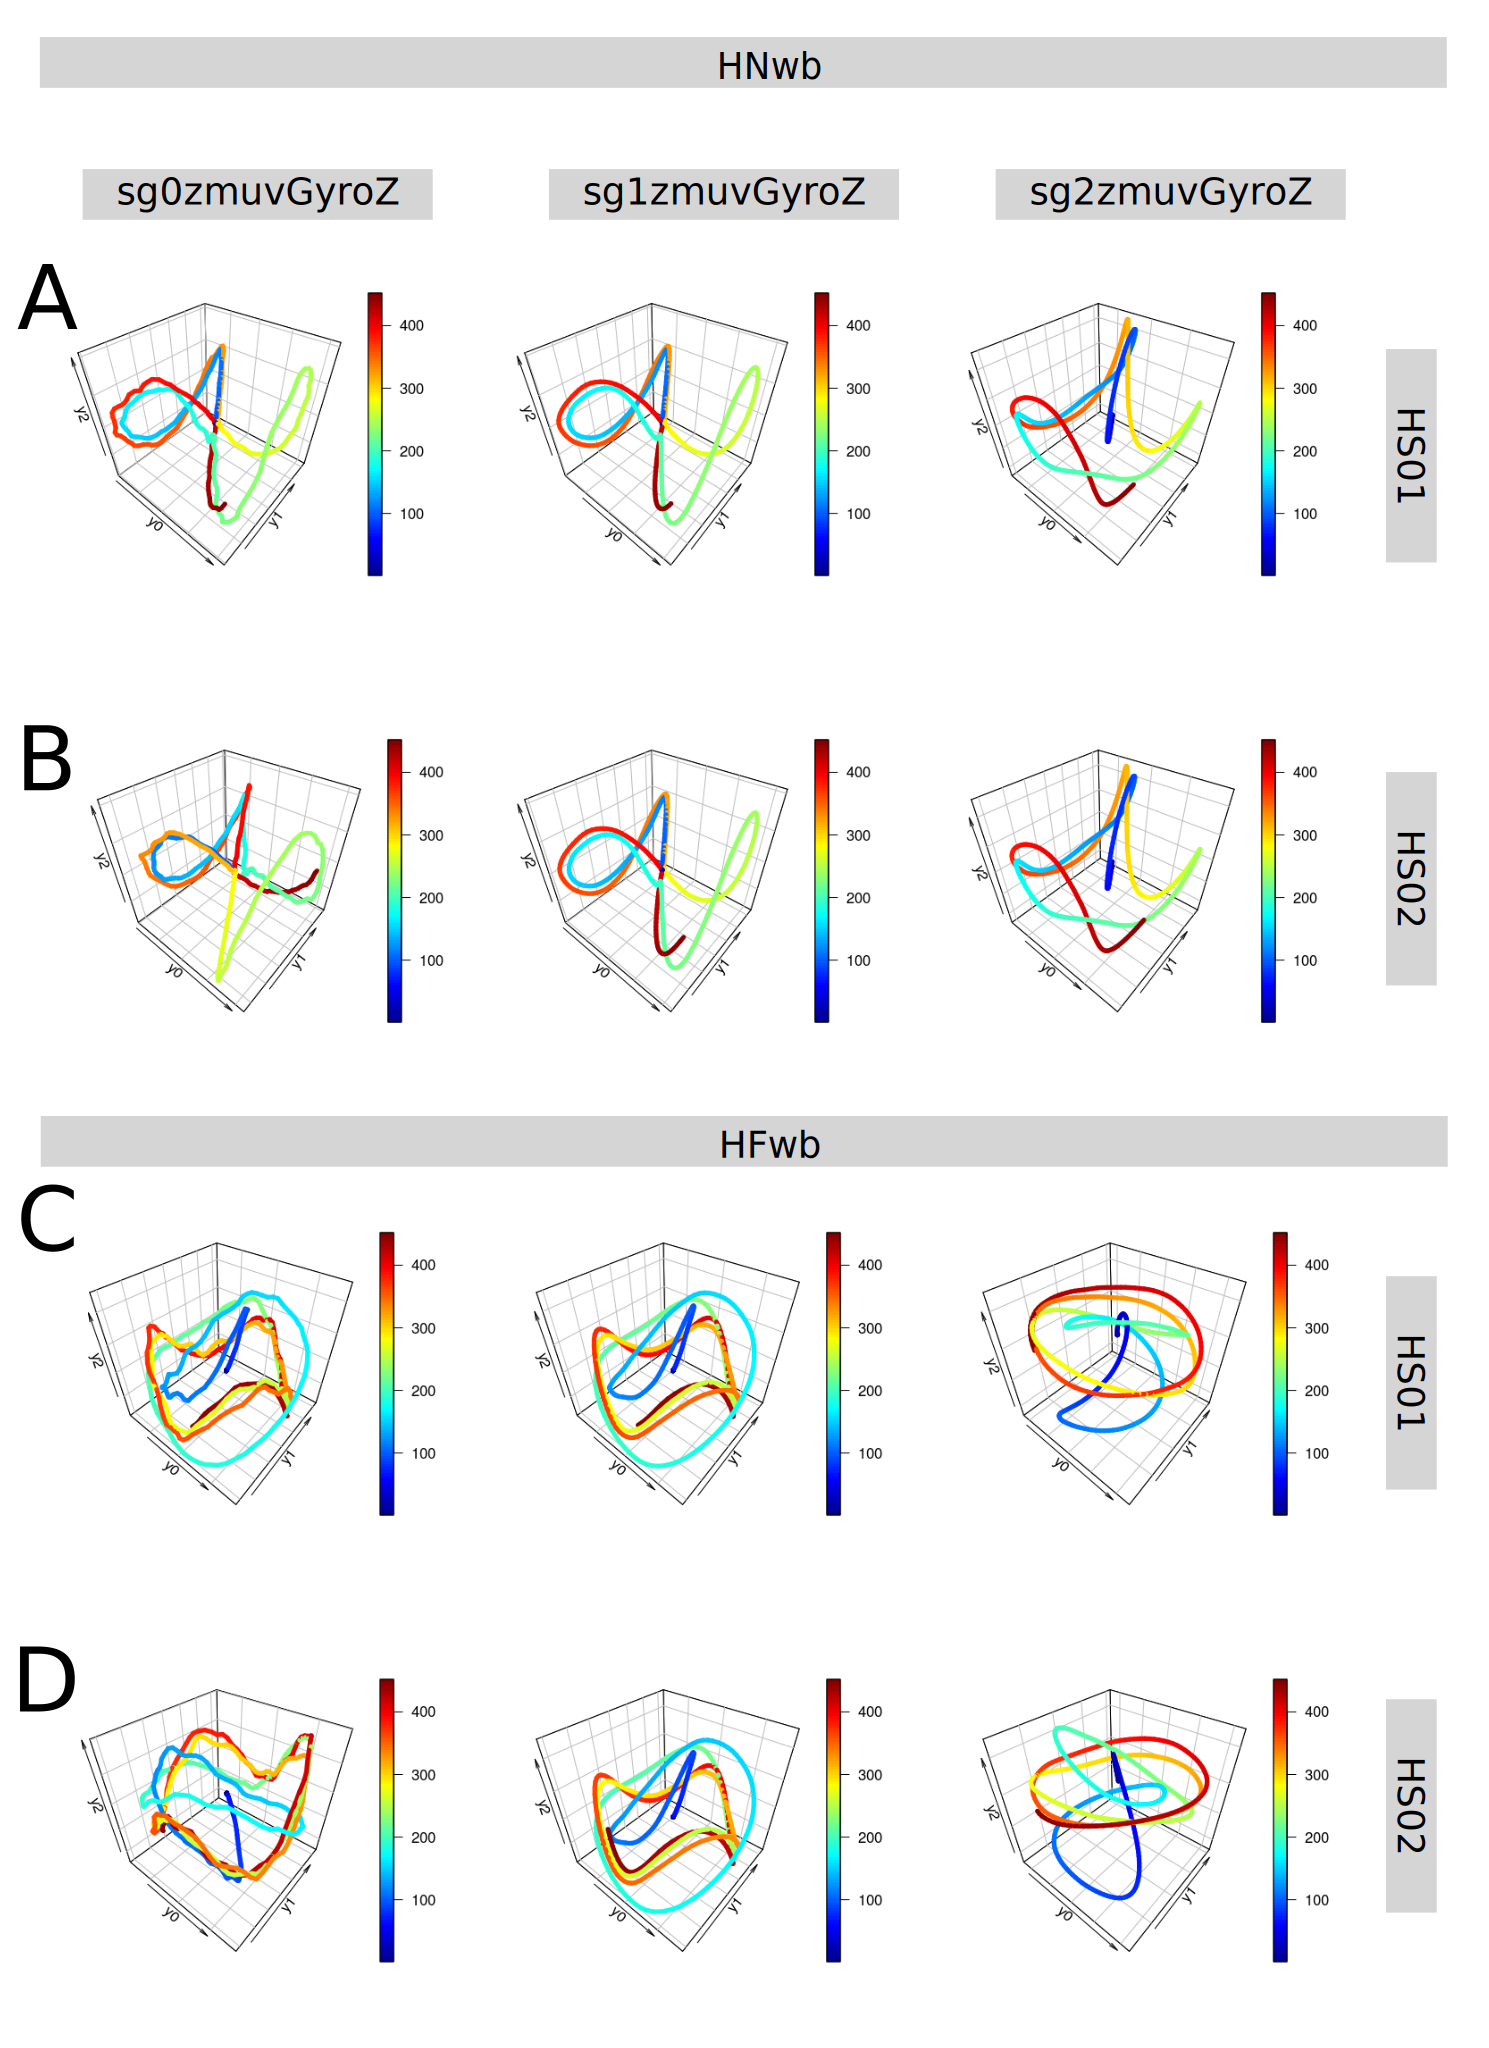
\includegraphics[height=0.8\textheight]{rss_Hwb_w500}
\caption{
	{\bf RSSs for horizontal arm movements (with beat).}
	Reconstructed state spaces of participant p01 for 
	(A, B) horizontal normal movements with beat (HNwb) and 
	(C, D) horizontal faster velocity with beat (HFwb).
	Time series for raw-normalised (sg0zmuvGyroZ), 
	normalised-smoothed 1 (sg1zmuvGyroZ) and 
	normalised-smoothed 2 (sg2zmuvGyroZ) with
	(A, C) sensor attached to the participant (HS01), and
	(B, D) sensor attached to the participant (HS02).	
	Reconstructed state spaces were computed with 
	embedding parameters $m=9$, $\tau=6$.
	R code to reproduce the figure is available from \cite{hwum2018}.
        }
     \label{fig:rss_Hwb_w500}
\end{figure}
%%---------------------------------(FIGURE)------------------------------------



%%---------------------------------(FIGURE)-------------------------------------
\begin{figure}[!h]
\centering
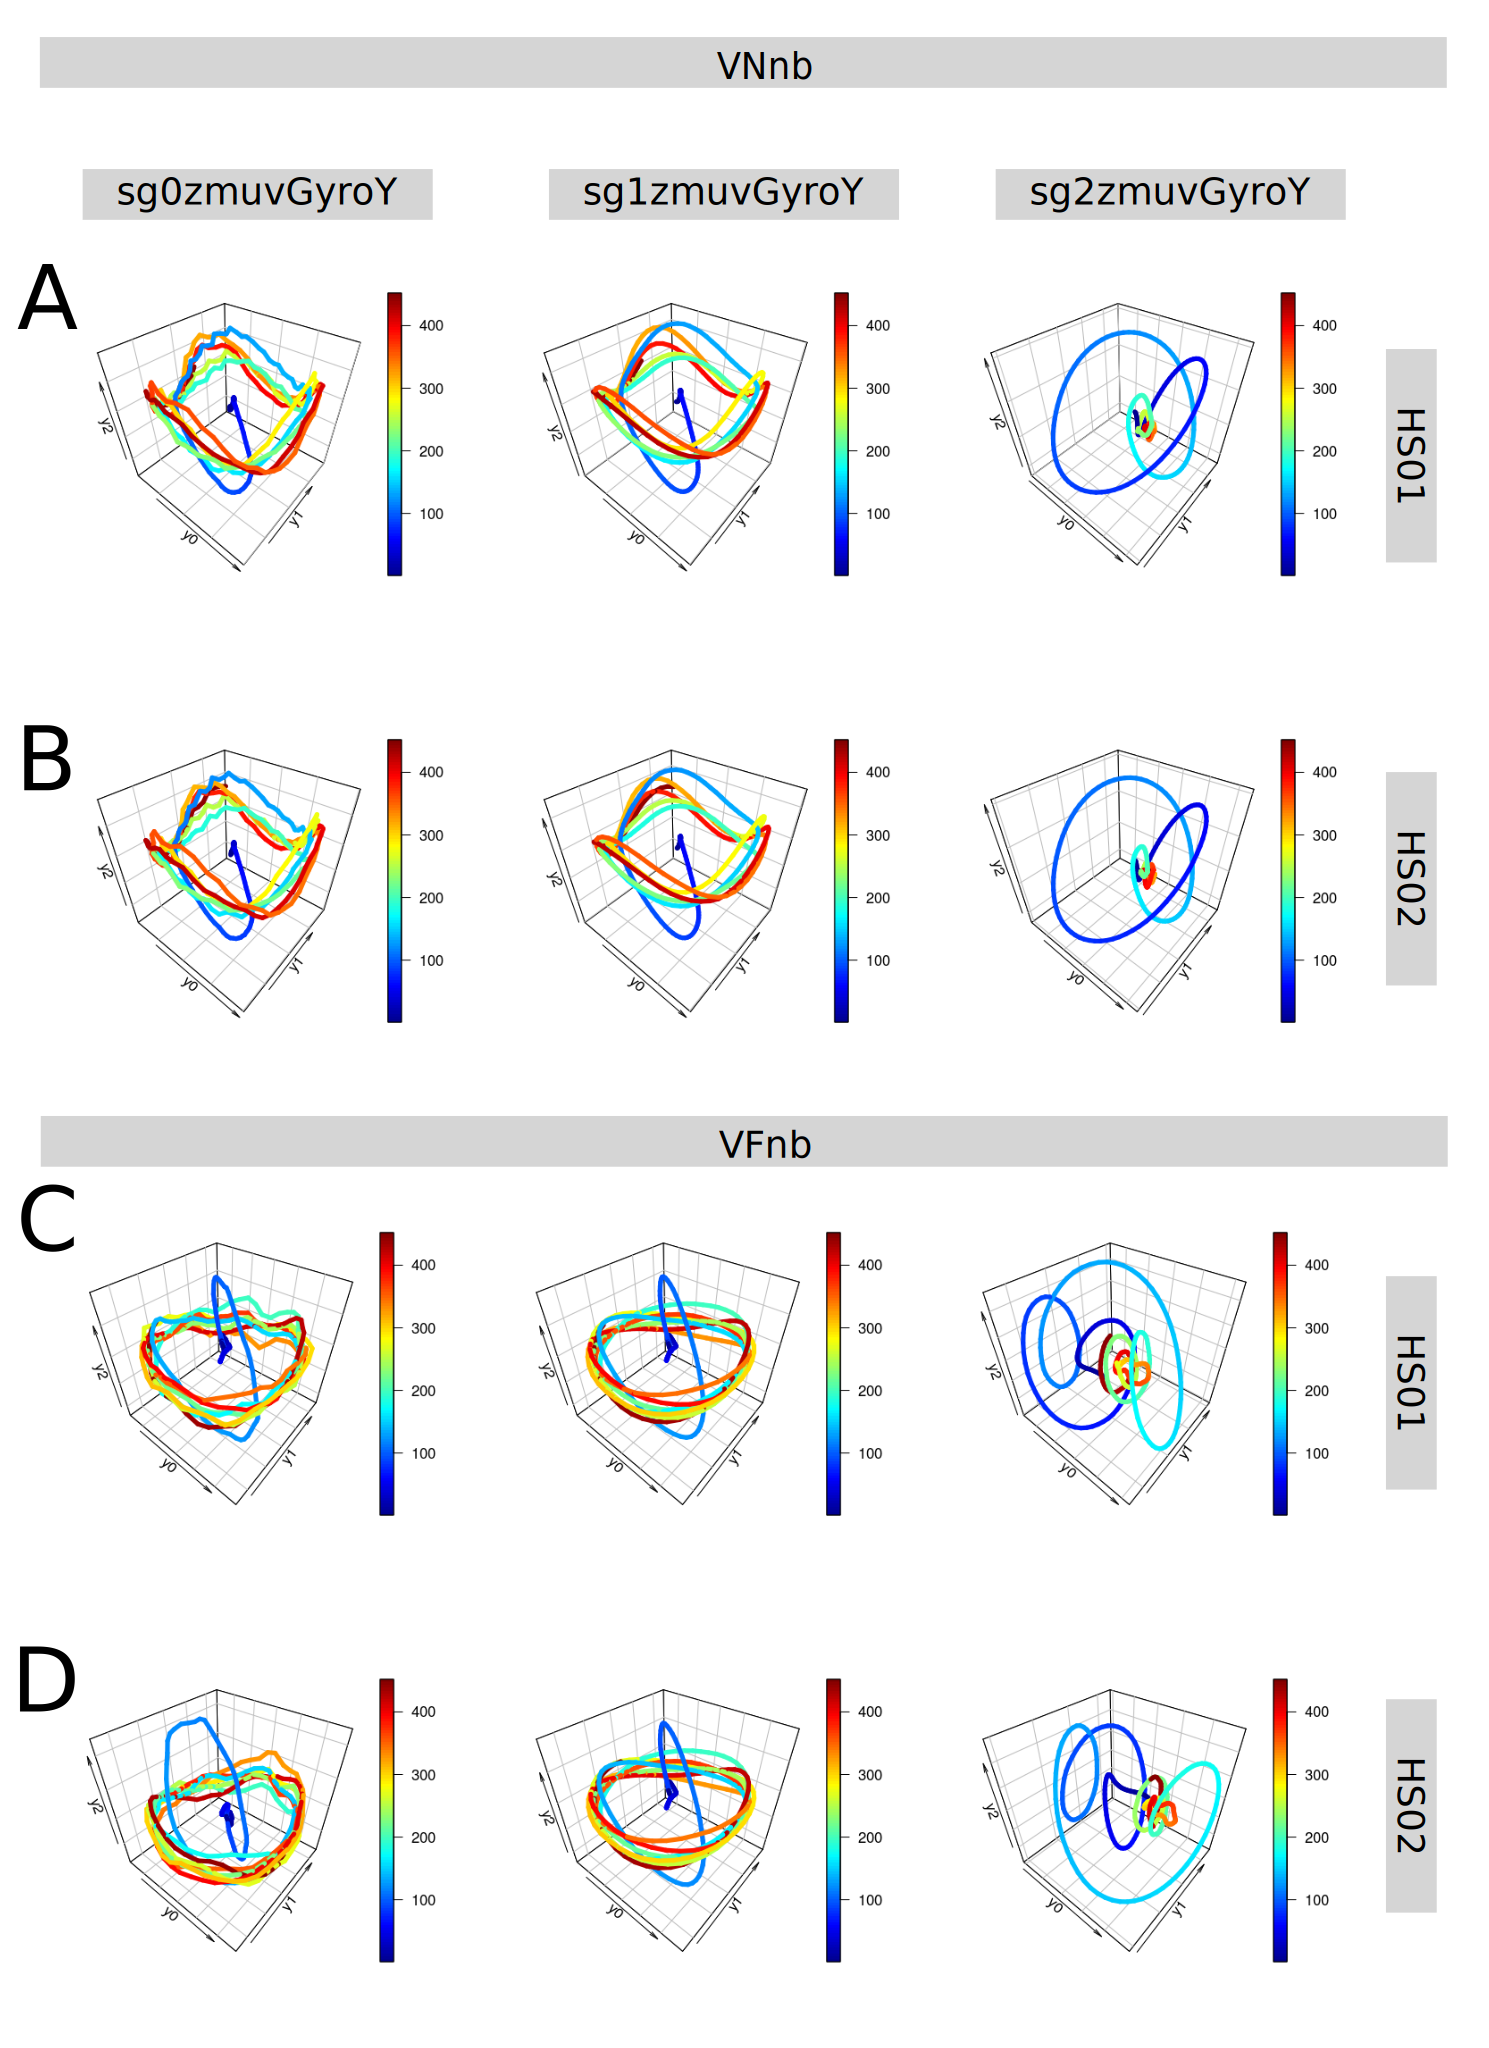
\includegraphics[height=0.8\textheight]{rss_Vnb_w500}
\caption{
	{\bf RSSs for vertical arm movements (no beat).}
	Reconstructed state spaces of participant p01 for 
	(A, B) vertical normal movements with no beat (VNnb) and 
	(C, D) vertical faster velocity with no beat (VFnb).
	Time series for raw-normalised (sg0zmuvGyroY), 
	normalised-smoothed 1 (sg1zmuvGyroY) and 
	normalised-smoothed 2 (sg2zmuvGyroY) with
	(A, C) sensor attached to the participant (HS01), and
	(B, D) sensor attached to the participant (HS02).	
	Reconstructed state spaces were computed with 
	embedding parameters $m=9$, $\tau=6$.
	R code to reproduce the figure is available from \cite{hwum2018}.
        }
     \label{fig:rss_Vnb_w500}
\end{figure}
%%---------------------------------(FIGURE)------------------------------------

%%---------------------------------(FIGURE)-------------------------------------
\begin{figure}[!h]
\centering
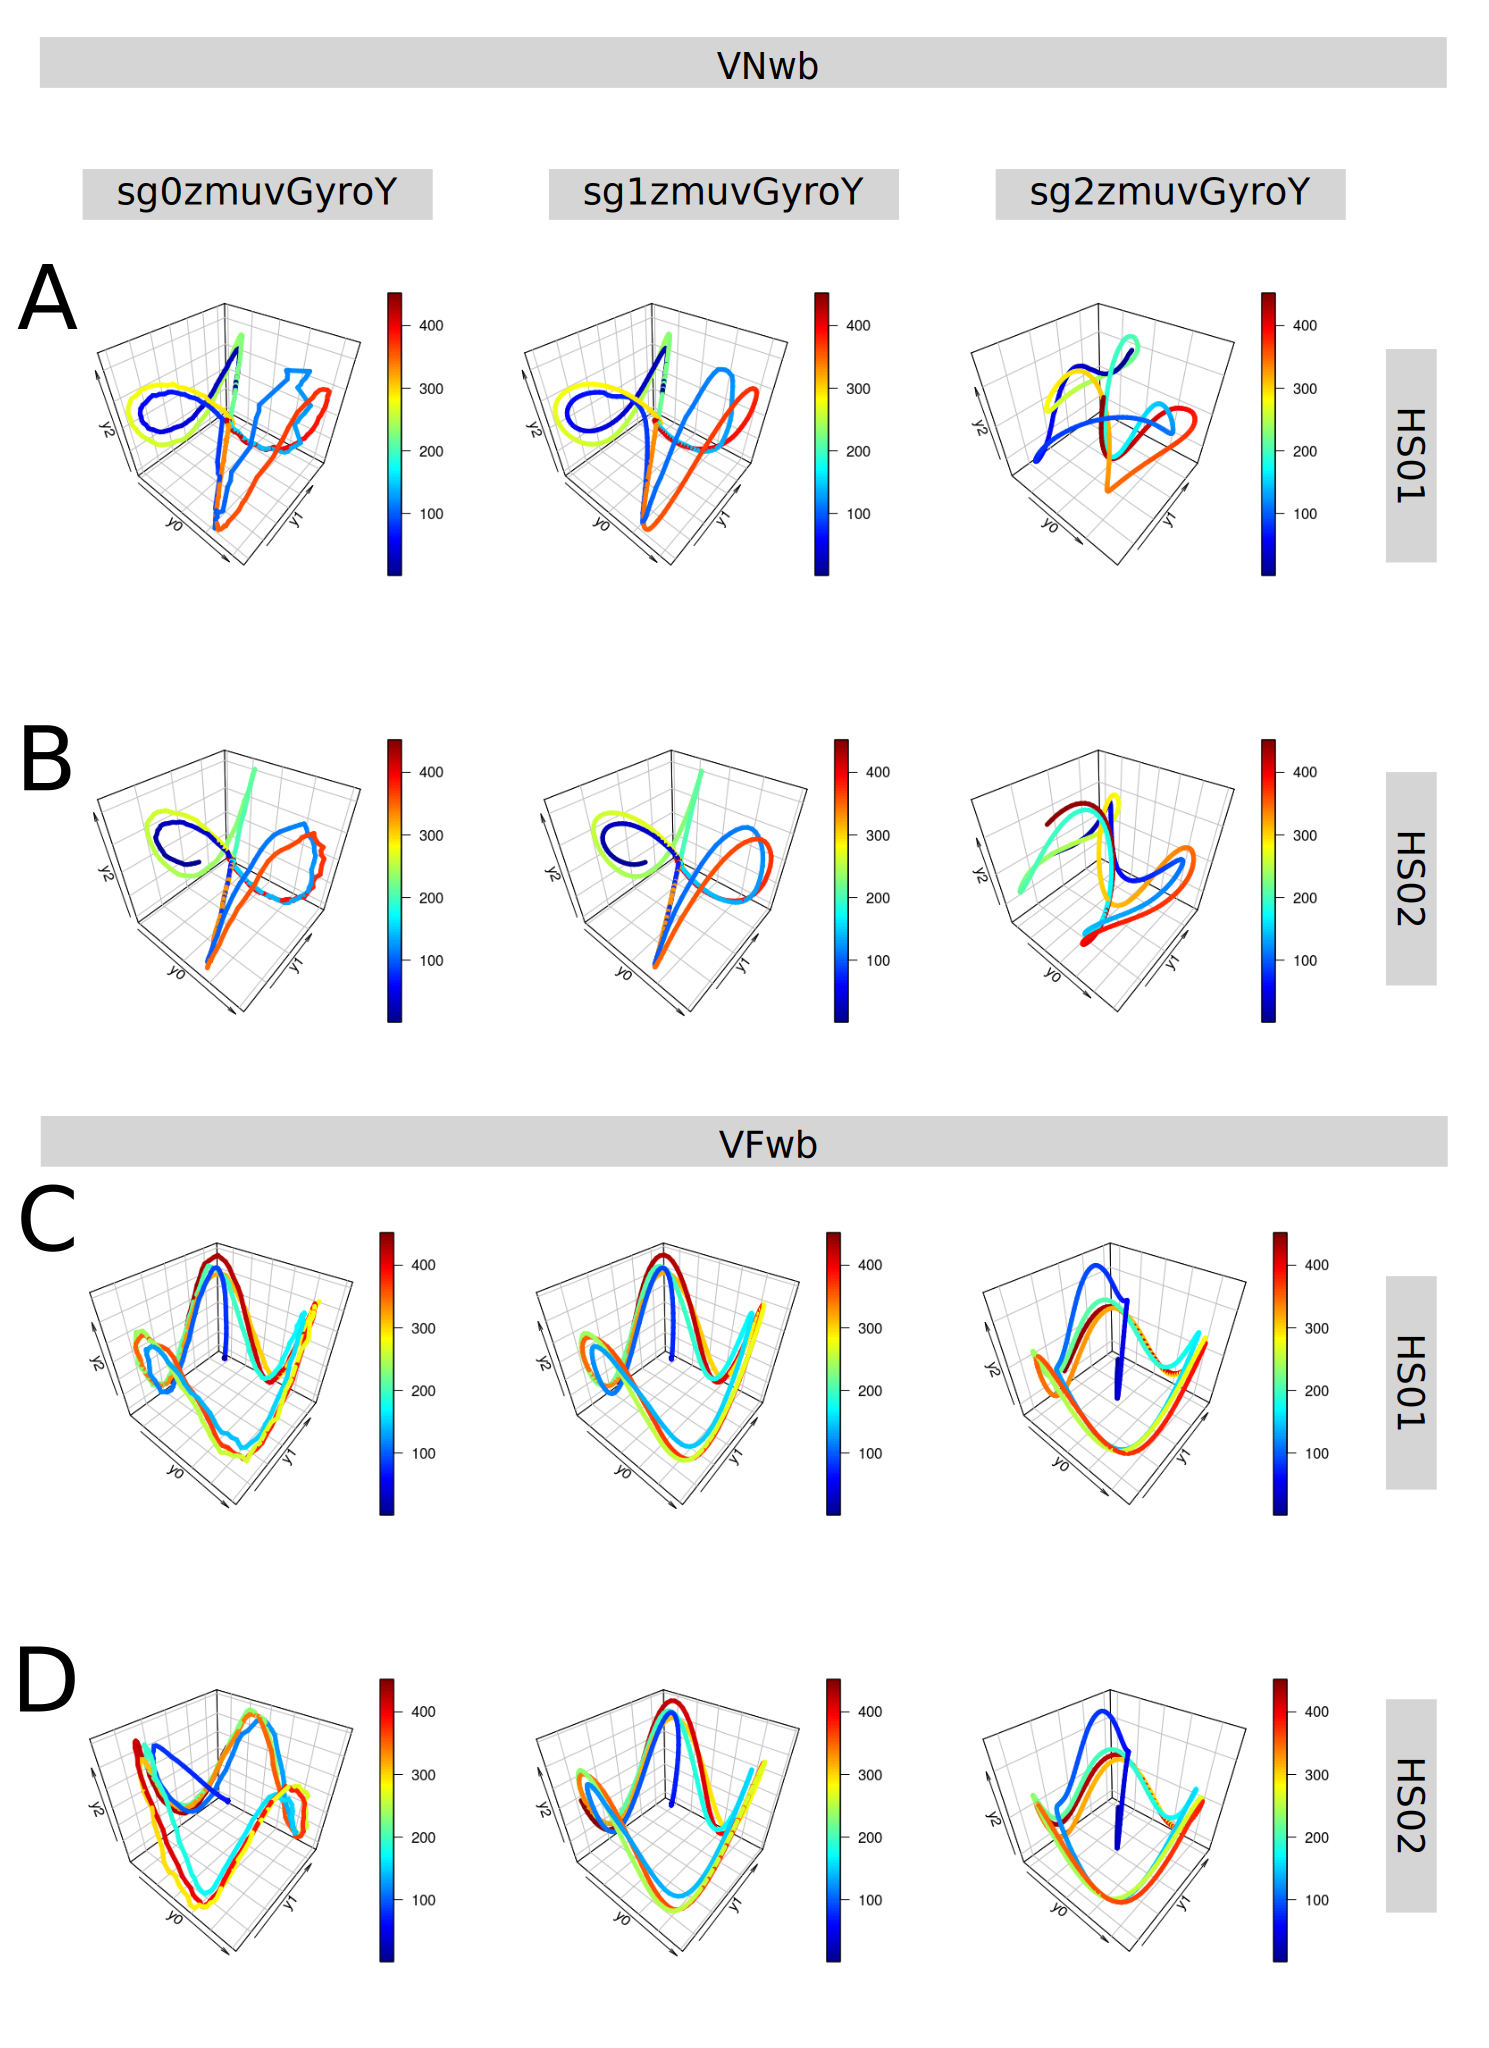
\includegraphics[height=0.8\textheight]{rss_Vwb_w500}
\caption{
	{\bf RSSs for vertical arm movements (with beat).}
	Reconstructed state spaces of participant p01 for 
	(A, B) vertical normal movements with beat (VNwb) and 
	(C, D) vertical faster velocity with beat (VFwb).
	Time series for raw-normalised (sg0zmuvGyroY), 
	normalised-smoothed 1 (sg1zmuvGyroY) and 
	normalised-smoothed 2 (sg2zmuvGyroY) with
	(A, C) sensor attached to the participant (HS01), and
	(B, D) sensor attached to the participant (HS02).	
	Reconstructed state spaces were computed with 
	embedding parameters $m=9$, $\tau=6$.
	R code to reproduce the figure is available from \cite{hwum2018}.
        }
     \label{fig:rss_Vwb_w500}
\end{figure}
%%---------------------------------(FIGURE)------------------------------------




\section{Recurrences Plots}
Considering the embedding parameters $m=9$, $\tau=6$ and a recurrence 
threshold $\epsilon=1$, we present in this section recurrence plots (RPs) for 
participant $p01$ for horizontal and vertical arm movements in normal 
and faster velocity with beat and no beat sound (Figs \ref{fig:rps_Hnb_w500}, 
\ref{fig:rps_Hwb_w500}, \ref{fig:rps_Vnb_w500} and \ref{fig:rps_Vwb_w500}).


Figs \ref{fig:rps_Hnb_w500} show recurrence plots for horizontal normal
and horizontal faster arm movements with no beat sound. 
For horizontal normal arm movements with no beat, patterns in 
RPs for sg0zmuvGyroZ and sg1zmuvGyroZ look similar, however
patterns in RPs for sg2zmuvGyroZ are different (Figs \ref{fig:rps_Hnb_w500}),
such behavior of RPs patterns is similar with regards to the smoothness 
presented in horizontal and faster arm movements with beat
(Fig \ref{fig:rps_Hwb_w500}).
With regards to the type of sensor, there is little visual differences in 
RPs patters, while patterns of RPs for different activities present diagonal 
lines that appear to be closer and more dense with horizontal faster
than horizontal normal arm movements (Fig \ref{fig:rps_Hnb_w500}).

Figs \ref{fig:rps_Hwb_w500} show patterns of RPs for horizontal normal
and faster arm movements while participants hear a beat. 
For these patterns in the RPs, the type activities for normal and 
faster arm movements can be easily noticed in the patterns,
as well as the change of smoothness between sg0zmuvGyroZ and sg1zmuvGyroZ
with the patterns for sg2zmuvGyroZ. It can also noted that there is 
little visual differences between the RP patters for sensor HS01 and 
HS02 (Figs \ref{fig:rps_Hwb_w500}).

Figs \ref{fig:rps_Vnb_w500} show patterns of RPs for vertical normal
and faster arm movements while no hearing a beat. One can note the 
the evidently differences of patterns between the levels of smoothness 
where, for instance, patterns of RPs from sg0zmuvGyroY and sg1zmuvGyroY 
looks similar while RPs for sg2zmuvGyroY are completely black.
Similarly, one can see little visual changes when comparing RPs patterns 
between sensors HS01 and HS02. 
However, the RPs patterns create a more dense presence of diagonal lines
for faster arm movements than normal arm movements 
(Figs \ref{fig:rps_Vnb_w500}).

Figs \ref{fig:rps_Vwb_w500} show RPs patterns for vertical normal and 
faster arm movements for participants hearing a beat. 
Patterns of RP for vertical normal and vertical faster arm movements are 
visually noticeable as well as the RPs patterns for changes in 
the increase of smoothness between sg0zmuvGyroY and sg1zmuvGyroY and 
with sg2zmuvGyroY. Once can also note that there is little visual 
changes of RPs patterns from different sensors (Figs \ref{fig:rps_Vwb_w500}).


%%---------------------------------(FIGURE)------------------------------------
\begin{figure}[!h]
\centering
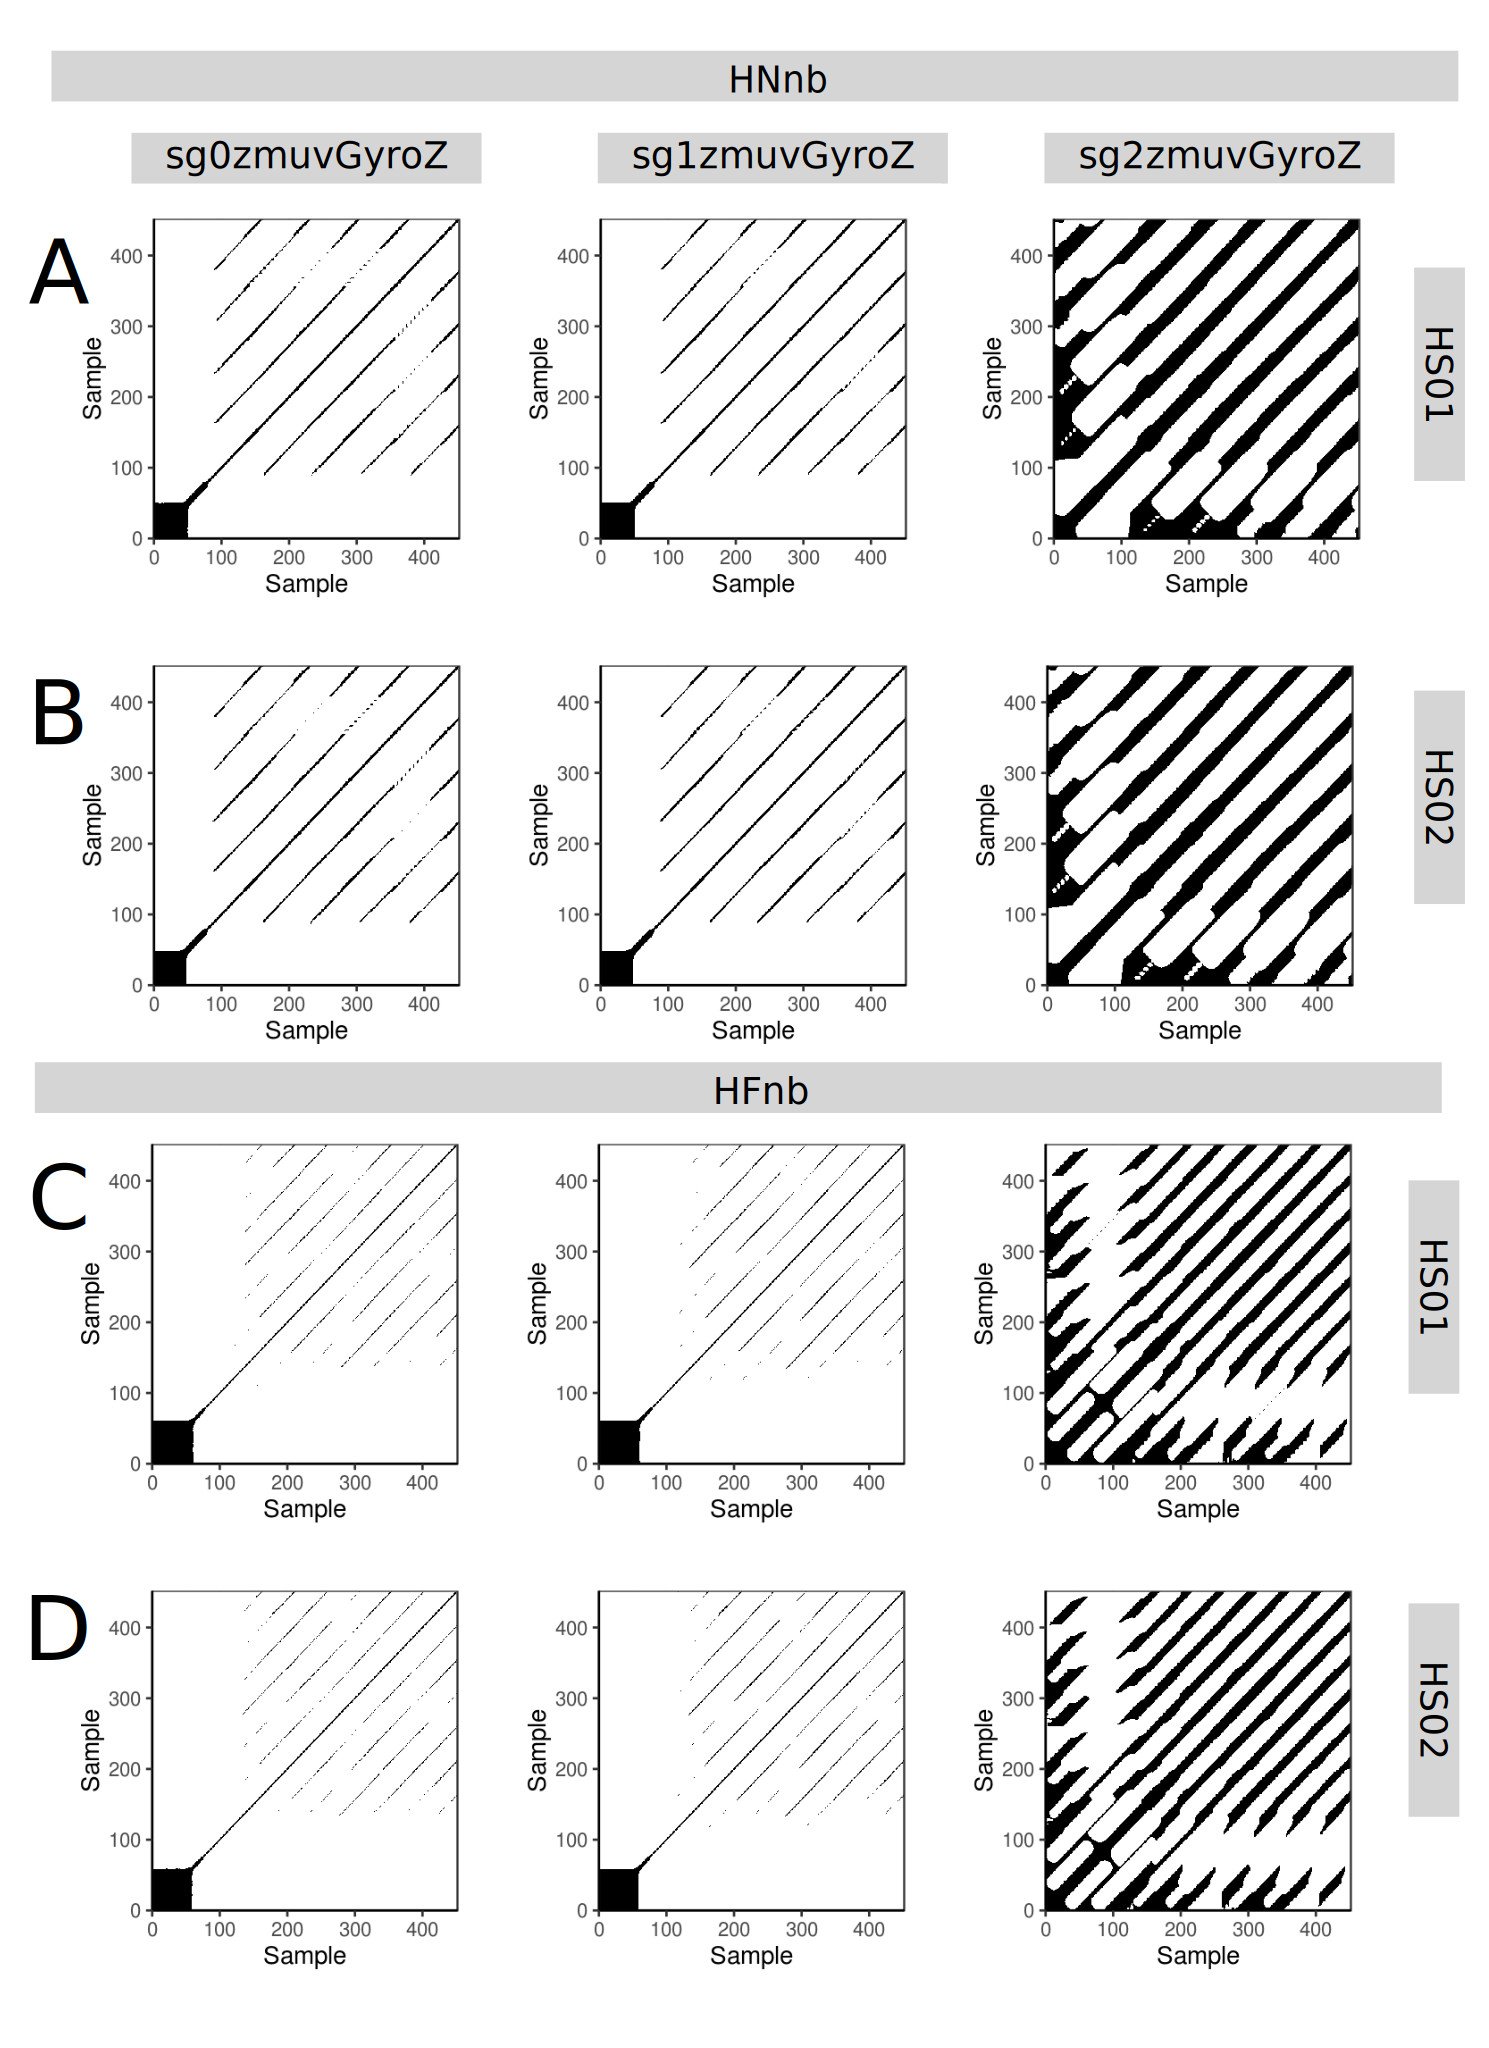
\includegraphics[height=0.8\textheight]{rps_Hnb_w500}
\caption{
	{\bf RPs for horizontal arm movements (no beat).}	
	Recurrence plots of participant p01 for 
	(A, B) horizontal normal movements with no beat (HNnb) and
	(C, D) horizontal faster movements with no beat (HFnb).
	Time series for raw-normalised (sg0zmuvGyroZ), 
	normalised-smoothed 1 (sg1zmuvGyroZ) and 
	normalised-smoothed 2 (sg2zmuvGyroZ) with
	(A, C) sensor 01 attached to the participant (HS01), and
	(B, D) sensor 02 attached to the participant (HS02).
	Recurrence plots were computed with 
	embedding parameters $m=9$, $\tau=6$ and 
	recurrence threshold $\epsilon=1$.
	R code to reproduce the figure is available from \cite{hwum2018}.
        }
    \label{fig:rps_Hnb_w500}
\end{figure}
%%---------------------------------(FIGURE)------------------------------------

%%---------------------------------(FIGURE)------------------------------------
\begin{figure}[!h]
\centering
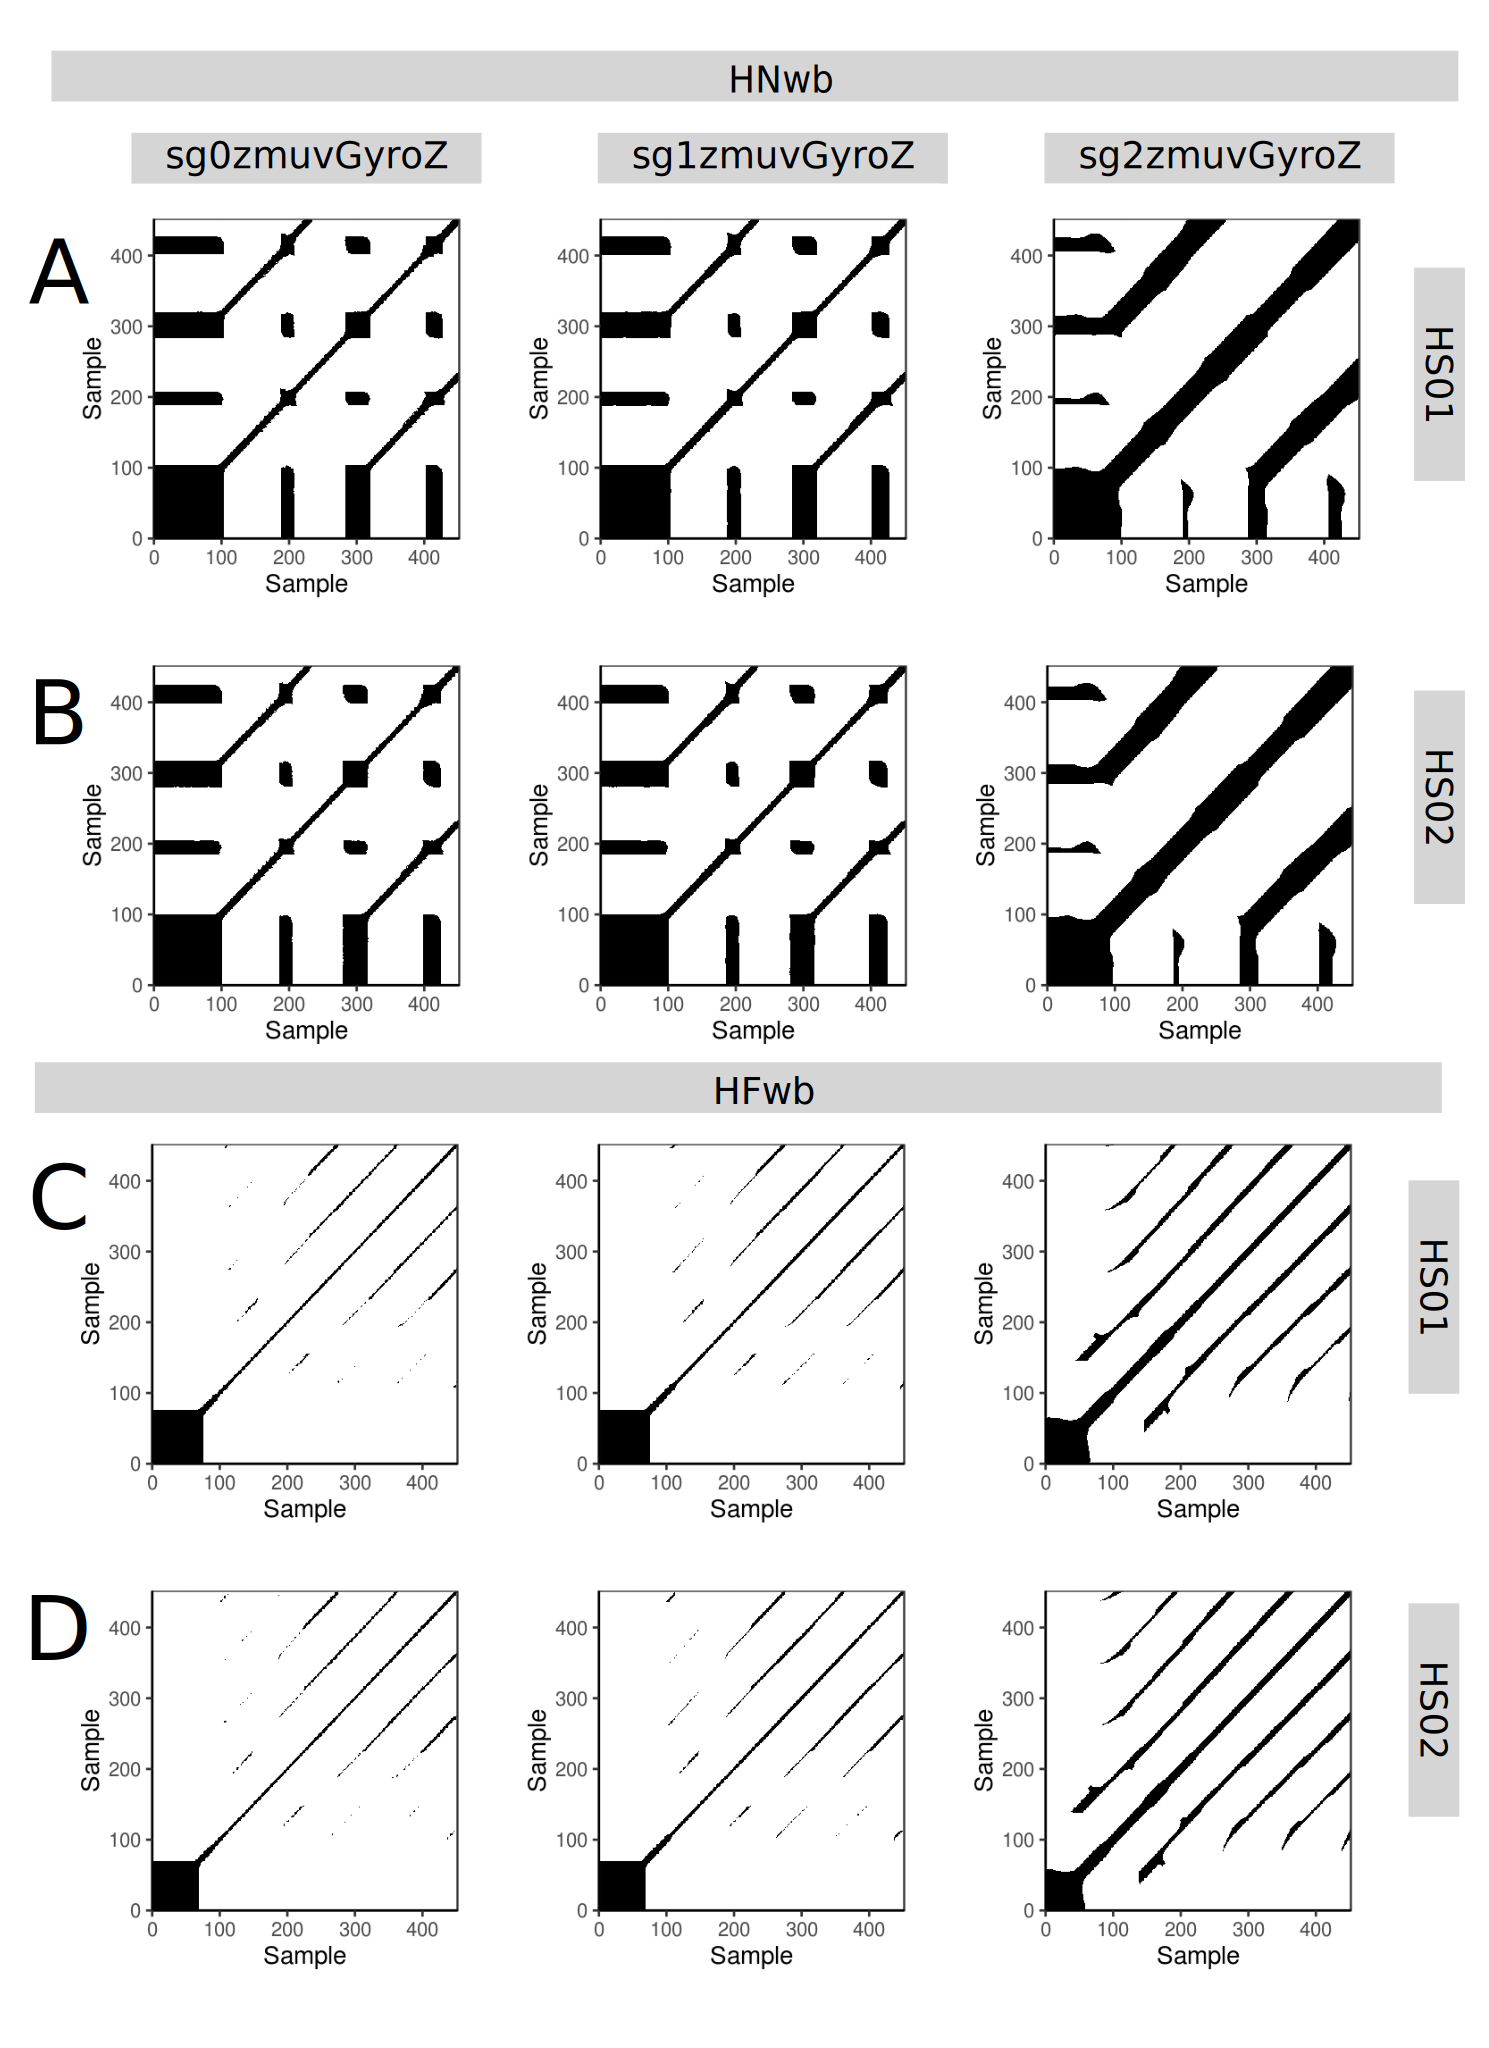
\includegraphics[height=0.8\textheight]{rps_Hwb_w500}
\caption{
	{\bf RPs for horizontal arm movements (with beat).}	
	Recurrence plots of participant p01 for 
	(A, B) horizontal normal movements with beat (HNwb) and
	(C, D) horizontal faster movements with beat (HFwb).
	Time series for raw-normalised (sg0zmuvGyroZ), 
	normalised-smoothed 1 (sg1zmuvGyroZ) and 
	normalised-smoothed 2 (sg2zmuvGyroZ) with
	(A, C) sensor 01 attached to the participant (HS01), and
	(B, D) sensor 02 attached to the participant (HS02).
	Recurrence plots were computed with 
	embedding parameters $m=9$, $\tau=6$ and 
	recurrence threshold $\epsilon=1$.
	R code to reproduce the figure is available from \cite{hwum2018}.
        }
    \label{fig:rps_Hwb_w500}
\end{figure}
%%---------------------------------(FIGURE)------------------------------------

%%---------------------------------(FIGURE)-----------------------------------
\begin{figure}[!h]
\centering
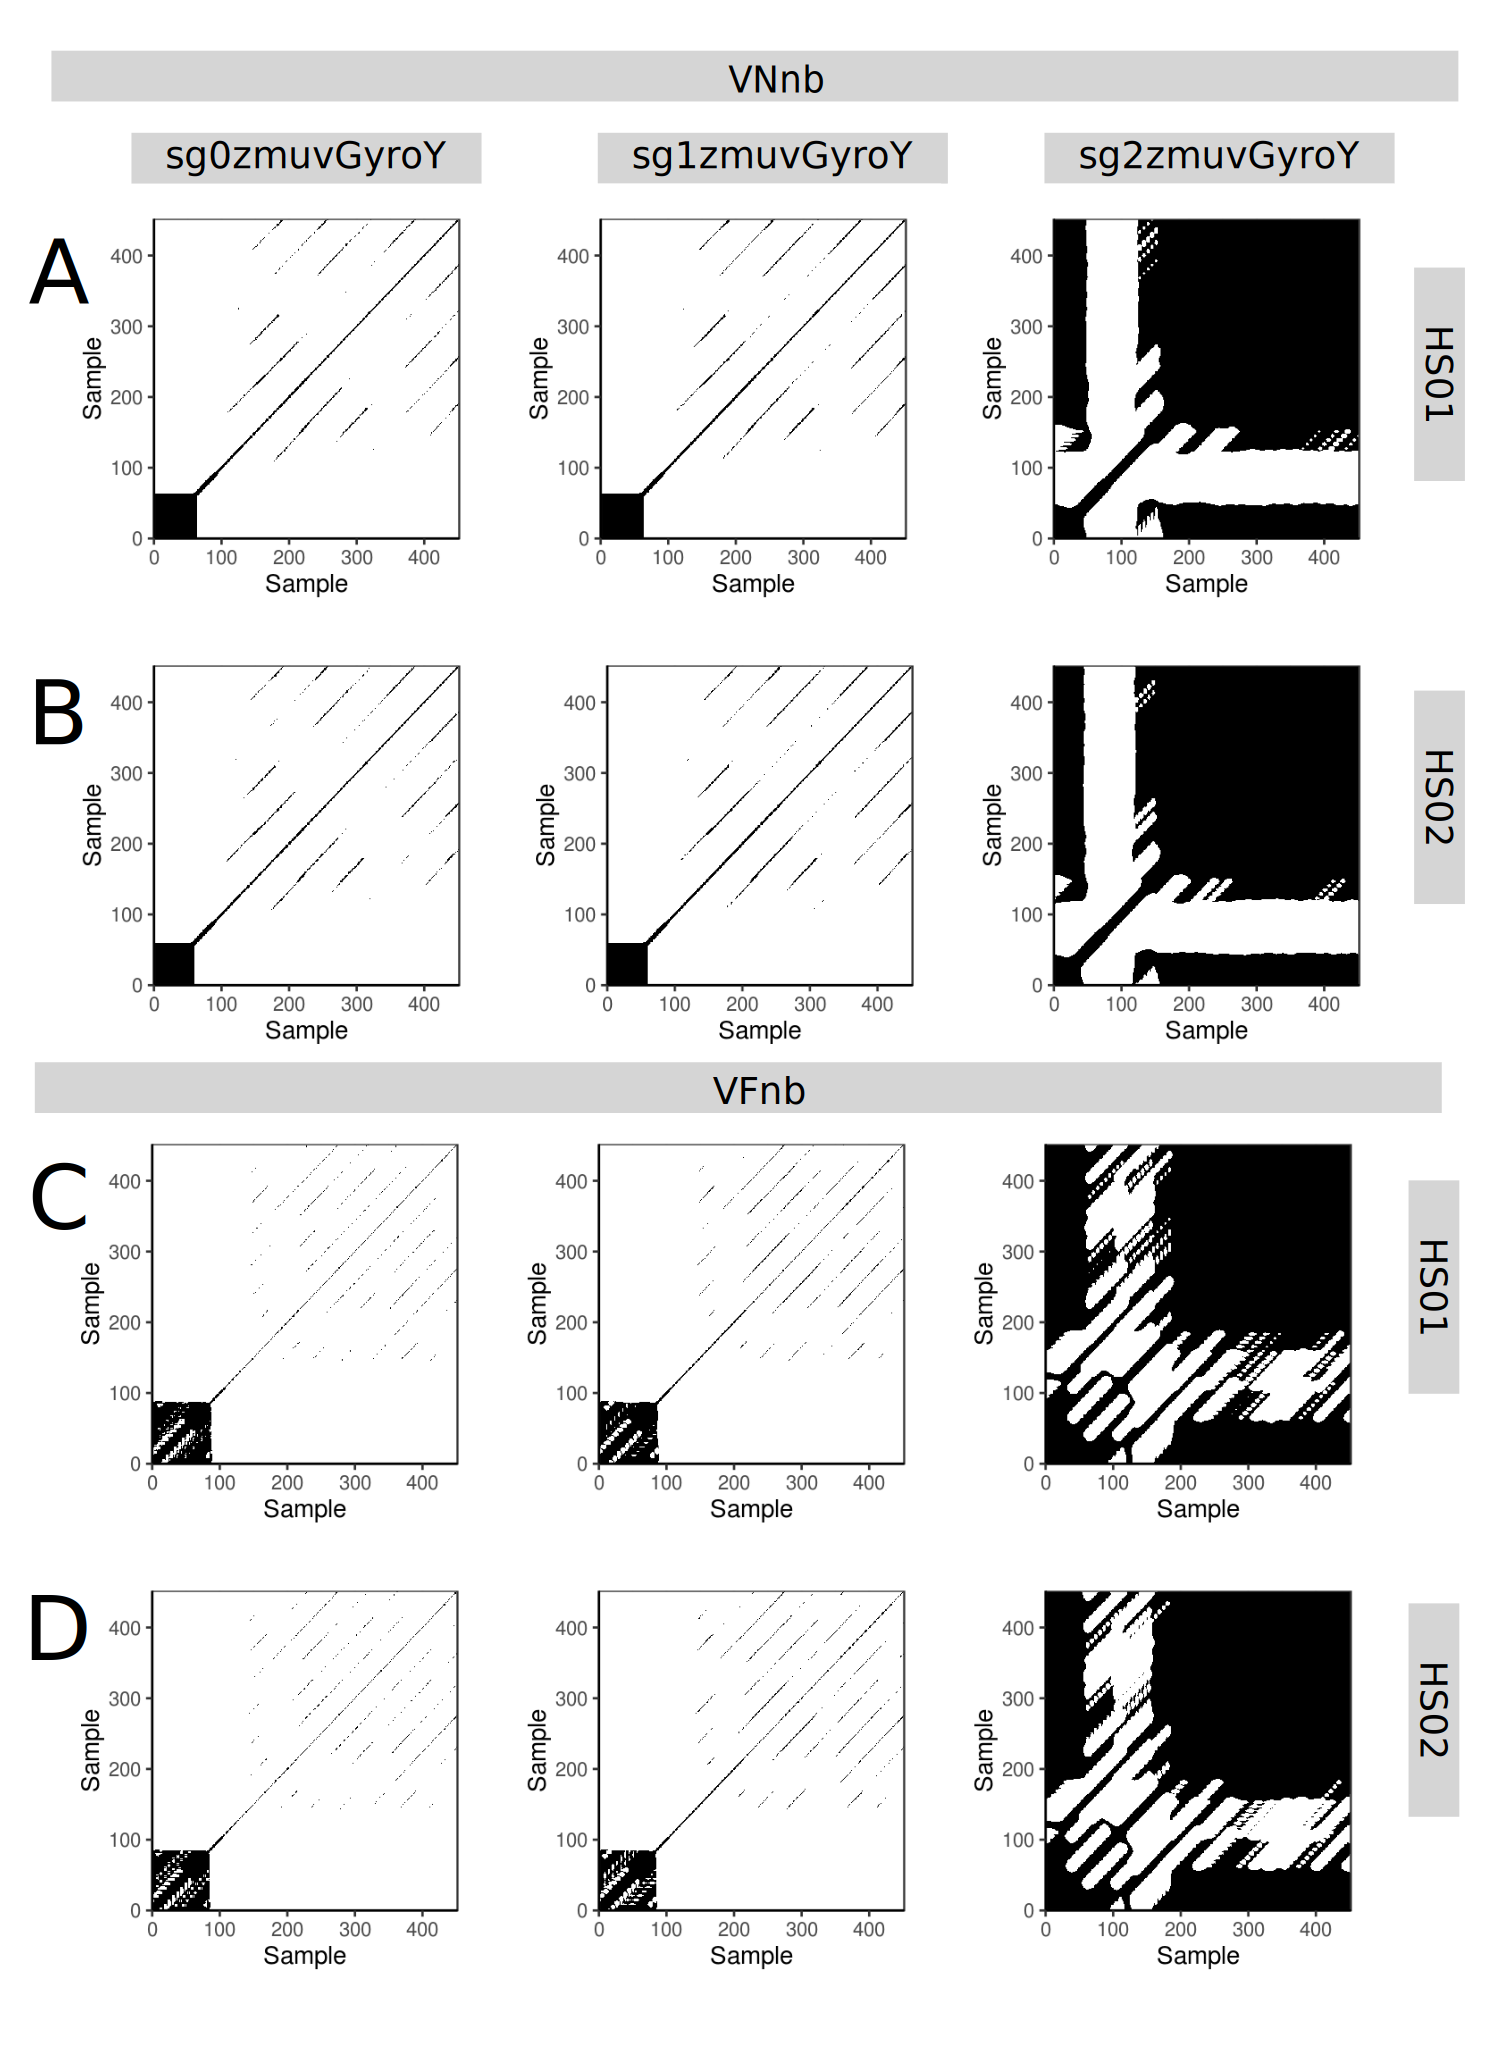
\includegraphics[height=0.8\textheight]{rps_Vnb_w500}
\caption{
	{\bf RPs for vertical arm movements (no beat).}	
	Recurrence plots of participant p01 for 
	(A, B) vertical normal movements with no beat (VNnb) and
	(C, D) vertical faster movements with no beat (VFnb).
	Time series for raw-normalised (sg0zmuvGyroY), 
	normalised-smoothed 1 (sg1zmuvGyroY) and 
	normalised-smoothed 2 (sg2zmuvGyroY) with
	(A, C) sensor 01 attached to the participant (HS01), and
	(B, D) sensor 02 attached to the participant (HS02).
	Recurrence plots were computed with 
	embedding parameters $m=9$, $\tau=6$ and 
	recurrence threshold $\epsilon=1$.
	R code to reproduce the figure is available from \cite{hwum2018}.
        }
    \label{fig:rps_Vnb_w500}
\end{figure}
%%---------------------------------(FIGURE)------------------------------------

%%---------------------------------(FIGURE)-----------------------------------
\begin{figure}[!h]
\centering
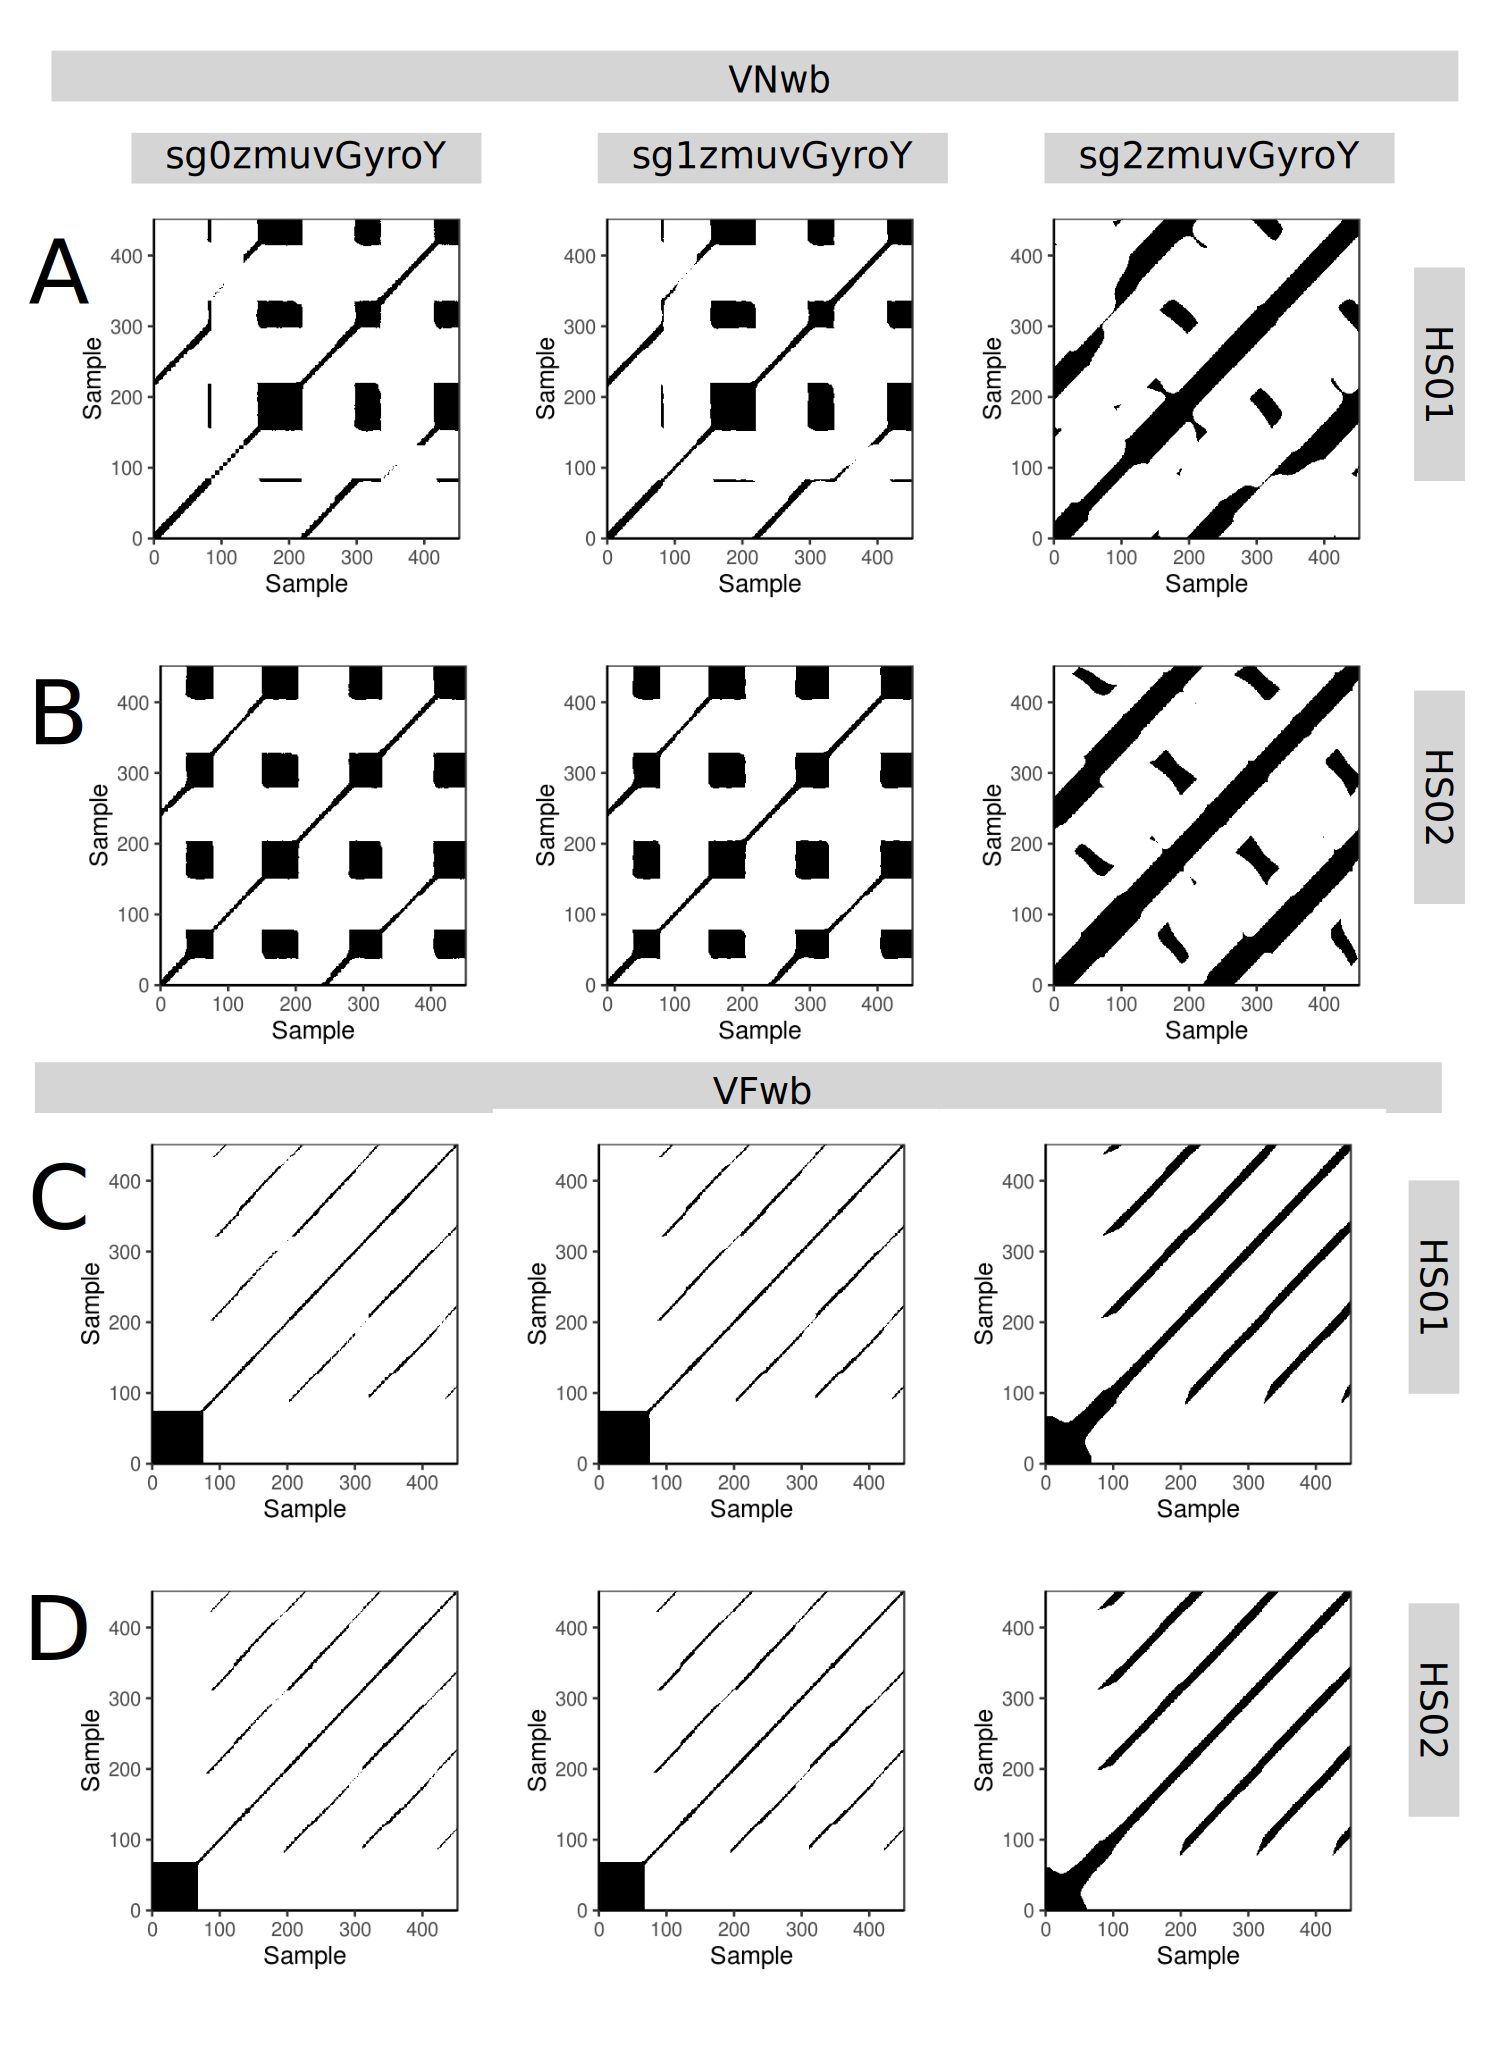
\includegraphics[height=0.8\textheight]{rps_Vwb_w500}
\caption{
	{\bf RPs for vertical arm movements (with beat).}	
	Recurrence plots of participant p01 for 
	(A, B) vertical normal movements with beat (VNwb) and
	(C, D) vertical faster movements with beat (VFwb).
	Time series for raw-normalised (sg0zmuvGyroY), 
	normalised-smoothed 1 (sg1zmuvGyroY) and 
	normalised-smoothed 2 (sg2zmuvGyroY) with
	(A, C) sensor 01 attached to the participant (HS01), and
	(B, D) sensor 02 attached to the participant (HS02).
	Recurrence plots were computed with 
	embedding parameters $m=9$, $\tau=6$ and 
	recurrence threshold $\epsilon=1$.
	R code to reproduce the figure is available from \cite{hwum2018}.
        }
    \label{fig:rps_Vwb_w500}
\end{figure}
%%---------------------------------(FIGURE)------------------------------------


\section{Recurrence Quantification Analysis}
In this section is shown Recurrence Quantification Analysis (RQA) metrics 
(REC, DET, RATIO and ENTR) for six participants ($p01, p04, p05, p10, p11, p15$)
for horizontal arm movements (HNnb, HNwb, HFnb, HFwb) 
and vertical arm movements (VNnb, VNwb, VFnb, VFwb)  
for sensors HS01 and HS02 with three smoothed time series 
(sg0zmuvGyro, sg1zmuvGyro and  sg2zmuvGyro).

\subsection{REC values}
Figs \ref{fig:rqa_rec_H} and \ref{fig:rqa_rec_V} show REC values,
representing the \% of black dots in the RPs, for vertical and horizontal 
arm movements.

It can be noted in Fig \ref{fig:rqa_rec_H} that REC values present 
little differences when comparing sensor HS01 and HS02. 
Similarly, considering the smoothness of the time series, REC values for 
participants appear to be similar in each of the activities 
(HNnb, HNwb, HFnb, HFwb) for sg0zmuvGyroZ and sg1zmuvGyroZ, 
while REC values for sg2zmuvGyroZ appear to fluctuate a bit more.
With regards to the type of activity, horizontal arm movements with beat 
(HNwb) appear to fluctuate more than other activities (HNnb, HFnb, HFwb). 
Also RET values appear to fluctuate more and be greater for faster
arm movements whereas RET values for normal arm movements appear 
to be constant (Fig \ref{fig:rqa_rec_H}).

Figs \ref{fig:rqa_rec_V} show RET values for vertical arm movements.
It can be noted that RET values appear to be similar for sensors HS01 and HS02
and the smoothness effect in REC values is more evident for sg2zmuvGyroY 
than REC values for sg0zmuvGyroY and sg1zmuvGyroY.
RET values appear to fluctuate more for vertical normal arm movements with 
beat (VNwb) than other activities (VNnb, VFnb, VFwb) and  RET values for 
VNnb, VFnb and VFwb appear to be constant and show little fluctuation 
between participants.
%%---------------------------------(FIGURE)------------------------------------
\begin{figure}[!h]
\centering
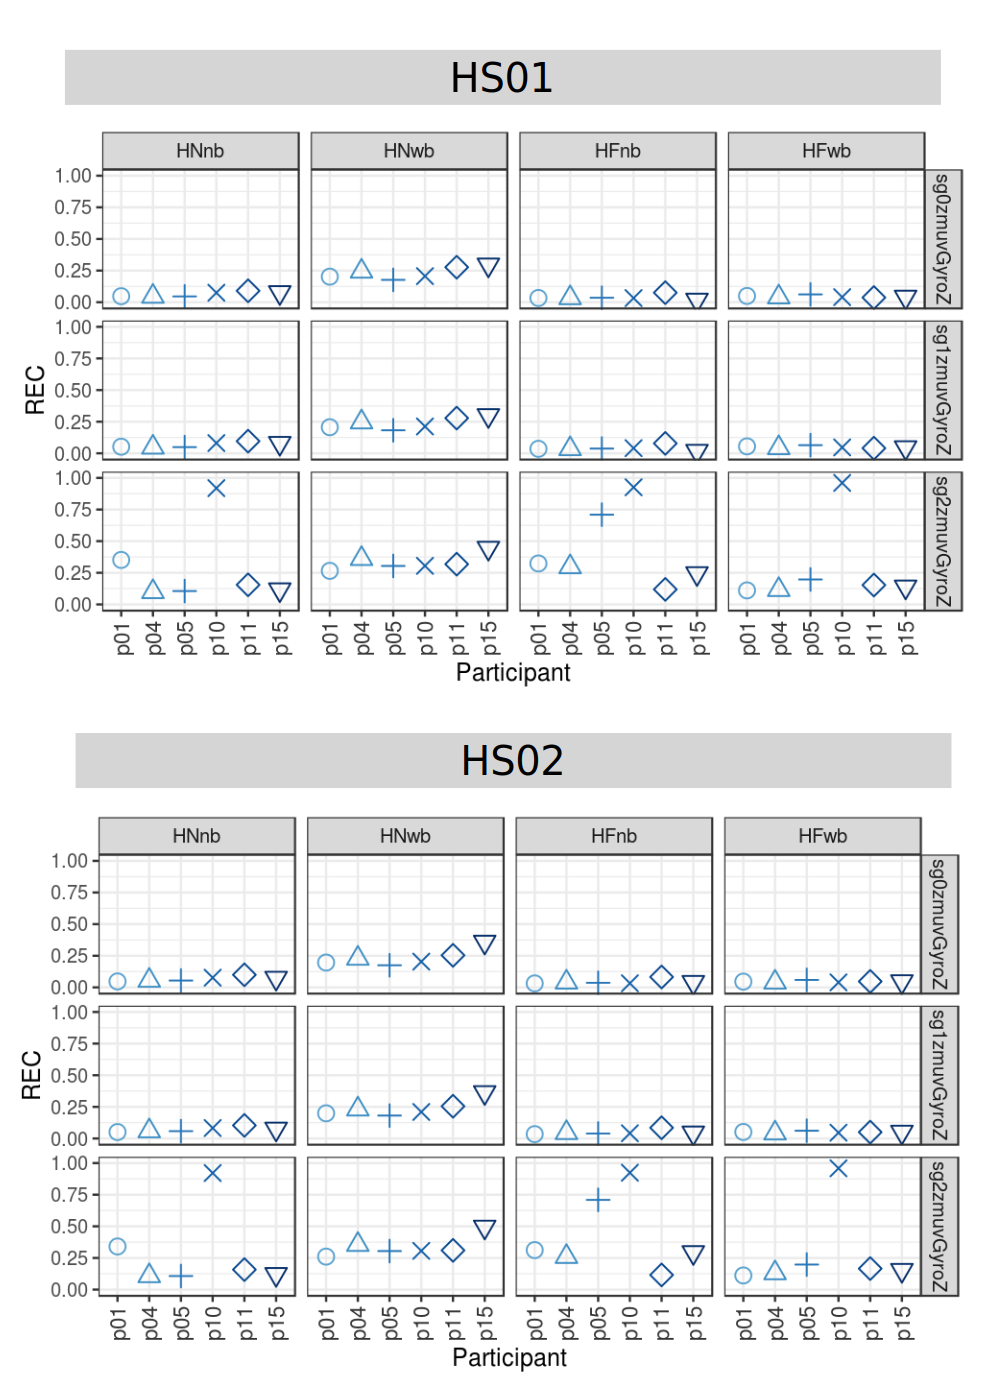
\includegraphics[width=0.9\textwidth]{rqa_rec_H_w500}
    \caption{
	{\bf REC values for horizontal arm movements.}	
	REC values (representing \% of black dots in the RPs) for 
	6 participants performing horizontal arm movements 
	(HNnb, HNwb, HFnb, HFwb)
	for sensors HS01, HS02 and three smoothed-normalised axis 
	of GyroZ (sg0zmuvGyroZ, sg1zmuvGyroZ and sg2zmuvGyroZ).
	REC values were computed with 
	embedding parameters $m=9$, $\tau=6$ and recurrence threshold
	$\epsilon=1$.
	R code to reproduce the figure is available from \cite{hwum2018}.
        }
    \label{fig:rqa_rec_H}
\end{figure}
%%---------------------------------(FIGURE)------------------------------------
%%---------------------------------(FIGURE)------------------------------------
\begin{figure}[!h]
\centering
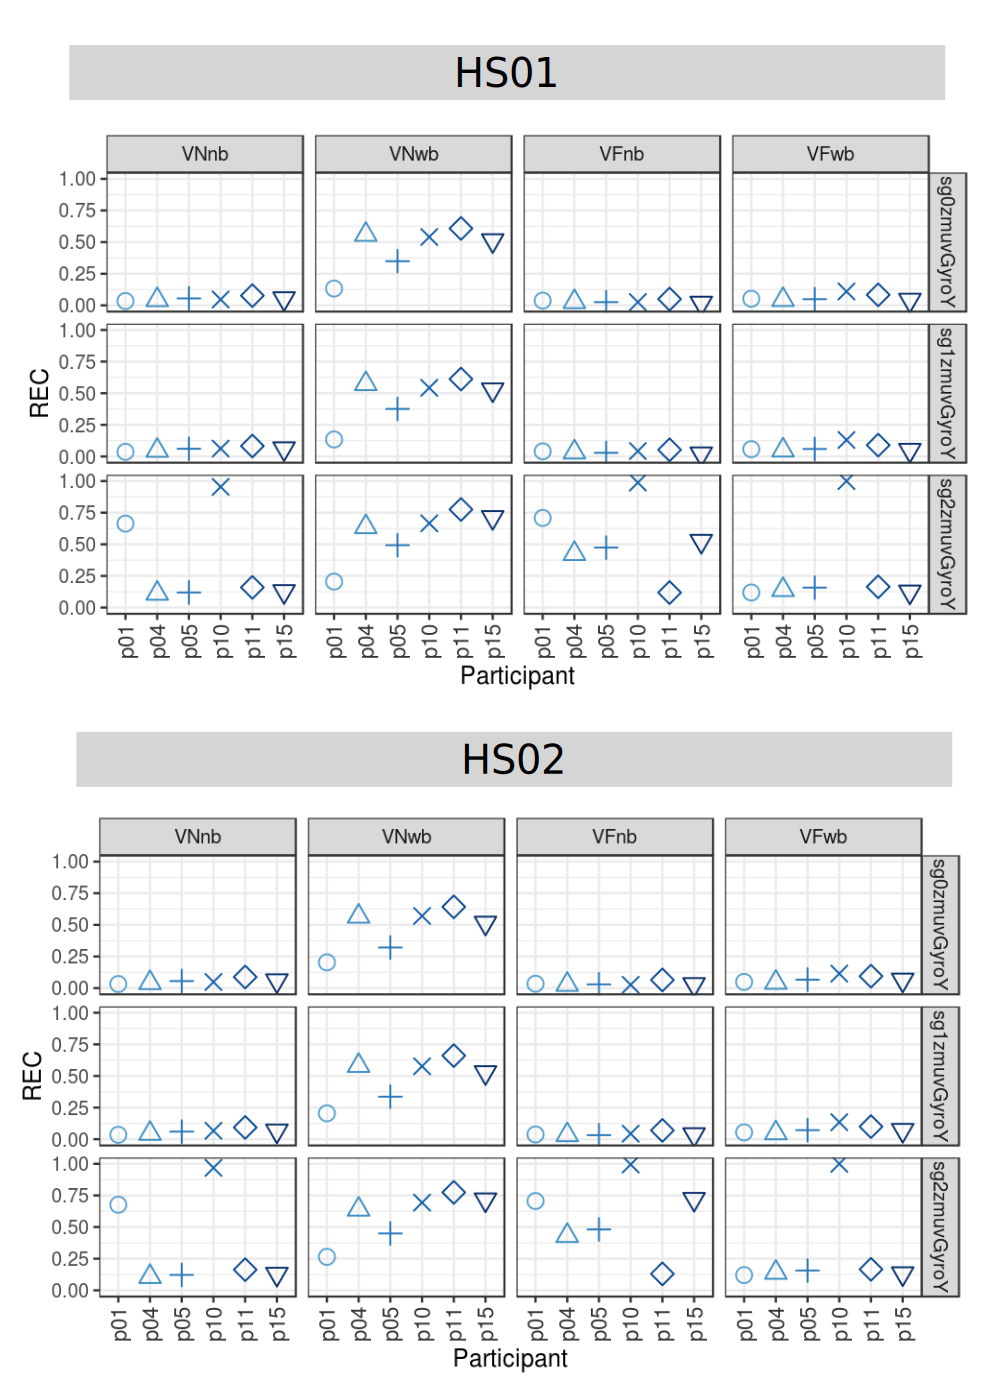
\includegraphics[width=0.9\textwidth]{rqa_rec_V_w500}
    \caption{
	{\bf REC values for vertical arm movements.}	
	REC values (representing \% of black dots in the RPs) for 
	6 participants performing vertical arm movements 
	(VNnb, VNwb, VFnb, VFwb)
	for sensors HS01, HS02 and three smoothed-normalised axis 
	of GyroZ (sg0zmuvGyroZ, sg1zmuvGyroZ and sg2zmuvGyroZ).
	REC values were computed with 
	embedding parameters $m=9$, $\tau=6$ and recurrence threshold
	$\epsilon=1$.
	R code to reproduce the figure is available from \cite{hwum2018}.
        }
    \label{fig:rqa_rec_V}
\end{figure}
%%---------------------------------(FIGURE)------------------------------------


\subsection{DET values}
DET values, representing predictability and organisation of the RPs, appear
to be constant for any source of time series 
(Figs \ref{fig:rqa_det_H} and \ref{fig:rqa_det_V}).
For both horizontal and vertical arm movements, the increase of smoothness 
of time series appear to affect the smoothness of DET values by making them 
to appear more similar as the smoothness increase.
Additionally, it can be noted more fluctuations of DET values 
for faster activities (HFnb, HFwb) 
than normal activities (HNnb, HNwb), specifically for  sg0zmuvGyroY 
(Figs \ref{fig:rqa_det_H}, \ref{fig:rqa_det_V}).


%%---------------------------------(FIGURE)------------------------------------
\begin{figure}[!h]
\centering
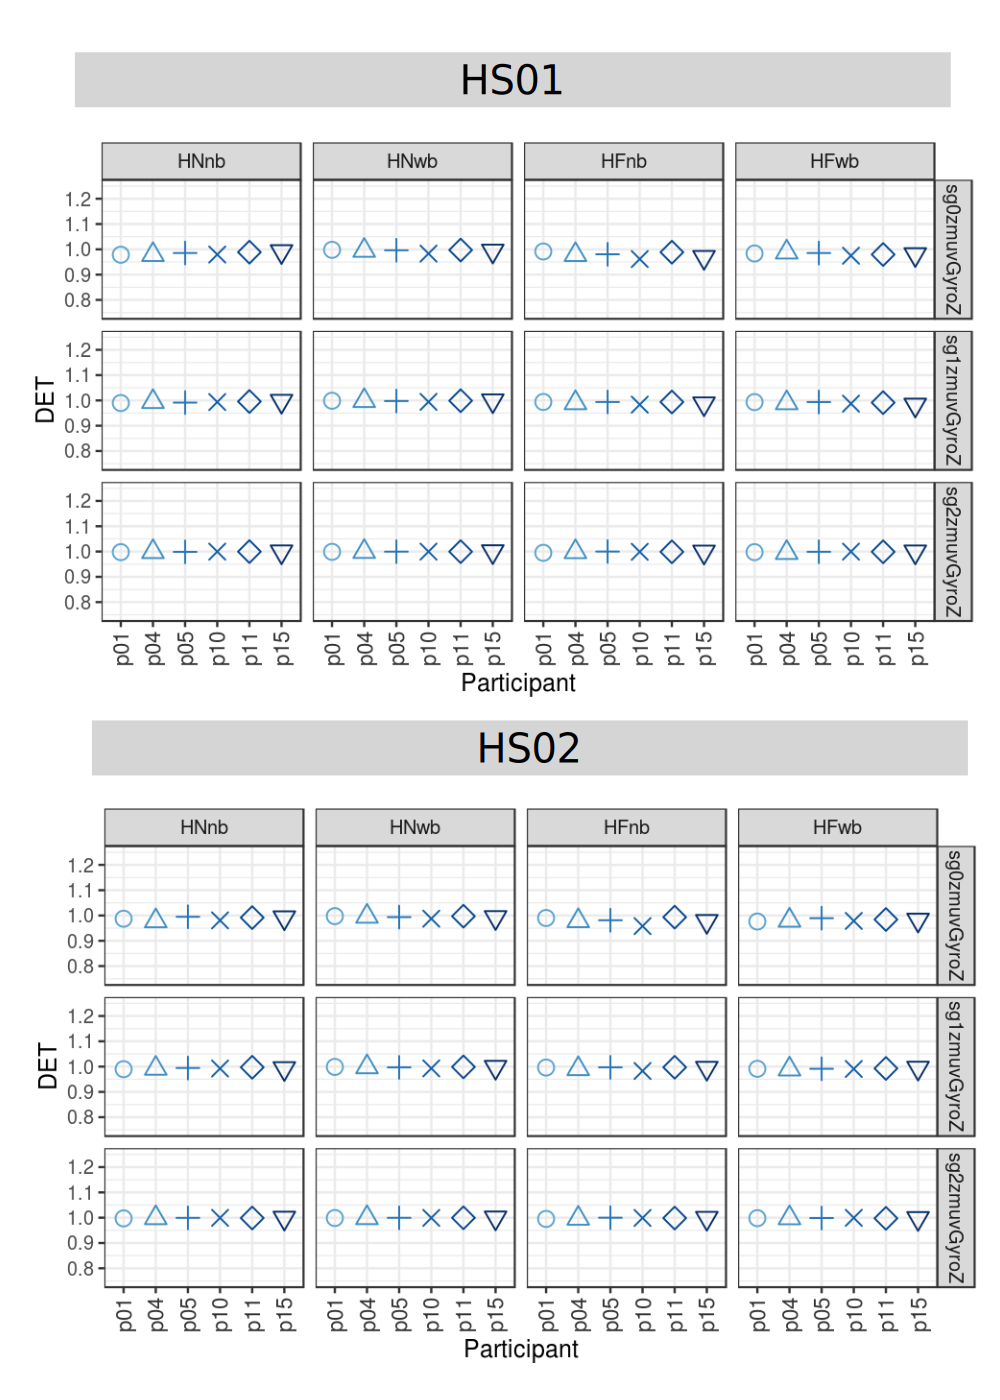
\includegraphics[width=0.9\textwidth]{rqa_det_H_w500}
    \caption{
	{\bf DET values for horizontal arm movements.}	
    	DET values (representing predictability and organisation of the RPs)
	for 6 participants performing horizontal arm movements 
	(HNnb, HNwb, HFnb, HFwb)
	for sensors HS01, HS02 and three smoothed-normalised axis 
	of GyroZ (sg0zmuvGyroZ, sg1zmuvGyroZ and sg2zmuvGyroZ).
	DET values were computed with 
	embedding parameters $m=9$, $\tau=6$ and recurrence threshold
	$\epsilon=1$.
	R code to reproduce the figure is available from \cite{hwum2018}.
        }
    \label{fig:rqa_det_H}
\end{figure}
%%---------------------------------(FIGURE)------------------------------------
%%---------------------------------(FIGURE)------------------------------------
\begin{figure}[!h]
\centering
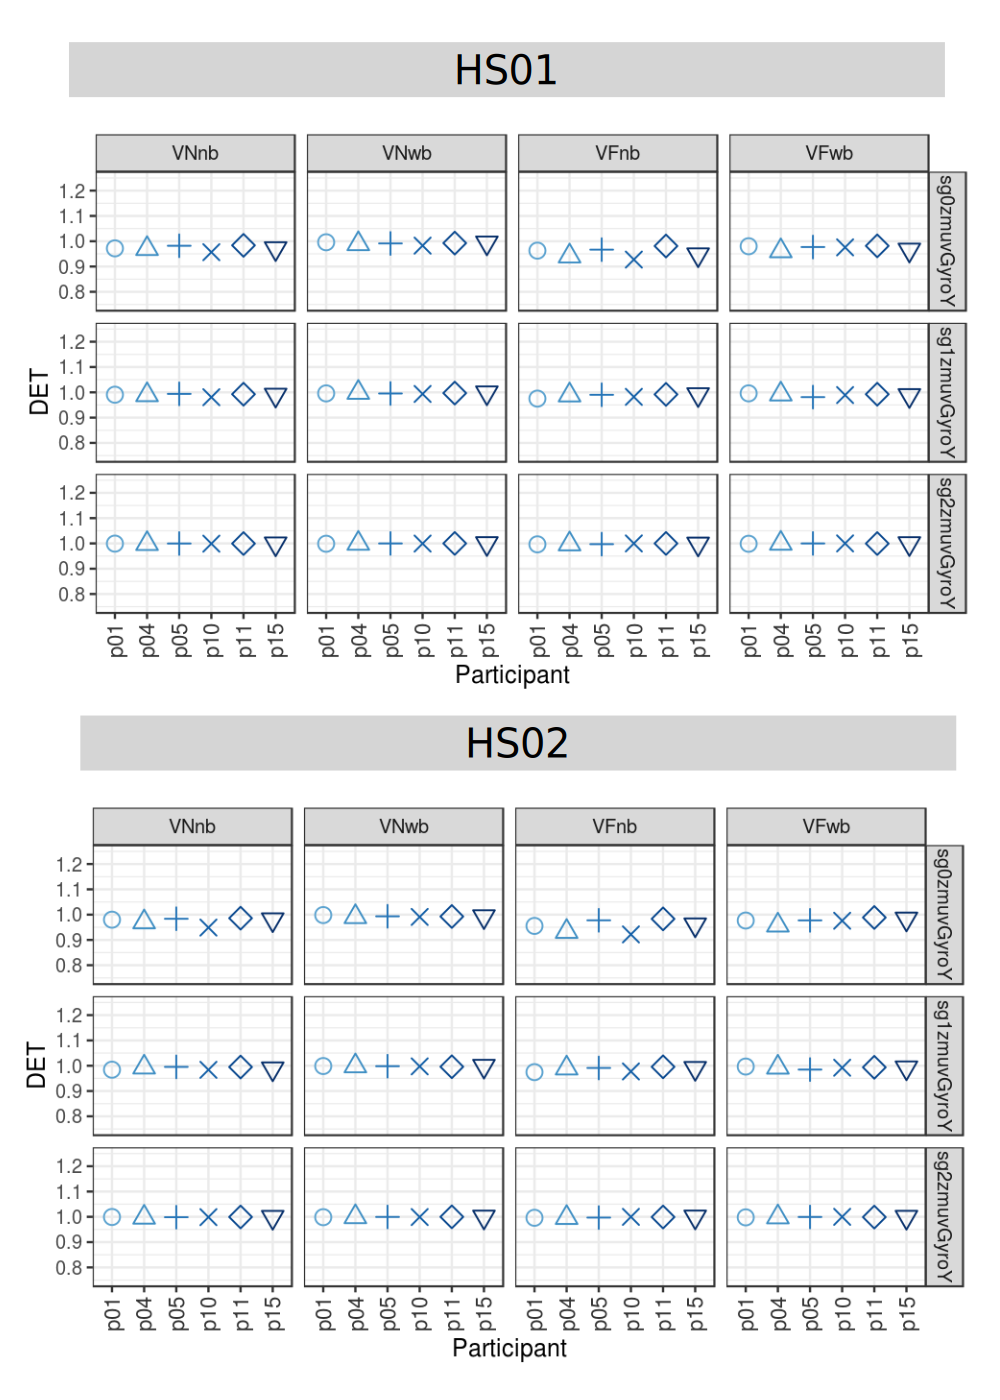
\includegraphics[width=0.9\textwidth]{rqa_det_V_w500}
    \caption{
	{\bf DET values for vertical arm movements.}	
    	DET values (representing predictability and organisation of the RPs)
	for 6 participants performing vertical arm movements 
	(VNnb, VNwb, VFnb, VFwb)
	for sensors HS01, HS02 and three smoothed-normalised axis 
	of GyroY (sg0zmuvGyroY, sg1zmuvGyroY and sg2zmuvGyroY).
	DET values were computed with 
	embedding parameters $m=9$, $\tau=6$ and recurrence threshold
	$\epsilon=1$.
	R code to reproduce the figure is available from \cite{hwum2018}.
        }
    \label{fig:rqa_det_V}
\end{figure}
%%---------------------------------(FIGURE)------------------------------------



\subsection{RATIO values}
RATIO values, representing dynamics transitions, for horizontal and 
vertical arm movements are shown in Figs \ref{fig:rqa_ratio_H} and 
\ref{fig:rqa_ratio_V}.

The fluctuation of RATIO values for horizontal faster arm movements 
appear to be more notable than RATIO values for horizontal normal arm 
movements. RATIO values appear to be constant for activity HNwb than
other activities (HNnb, HFnb, HFwb).
Regarding the smoothness of time series, RATIO values appear to have 
similar values for sg0zmuvGyroZ and sg1zmuvGyroZ while RATIOS values 
are more uniform for sg2zmuvGyroZ.
With regards to type of sensor, 
RET values appear to be similar for HS01 and HS02 with the exception of
$p15$ in HFnb activity (Figs \ref{fig:rqa_ratio_H}).

Figs \ref{fig:rqa_ratio_V} show RATIO values for vertical arm movements.
The fluctuation of RATIO values appears to be constant for the activity 
VNwb whereas other RATIO values for other activities (VNnb, VFnb, VFwb) 
appear to fluctuate more.
The smoothness of the time series affects only the RATIO values for 
sg2zmuvGyroY as these appear to be constant, while RET values for 
sg0zmuvGyroY and sg1zmuvGyroZ appear to have the similar RATIO values.
Additionally, RATIO values for type of sensors HS01 and HS02 appear 
to show similar values as well, with the exception of $p15$ in the 
VFnb activity.

%%---------------------------------(FIGURE)------------------------------------
\begin{figure}[!h]
\centering
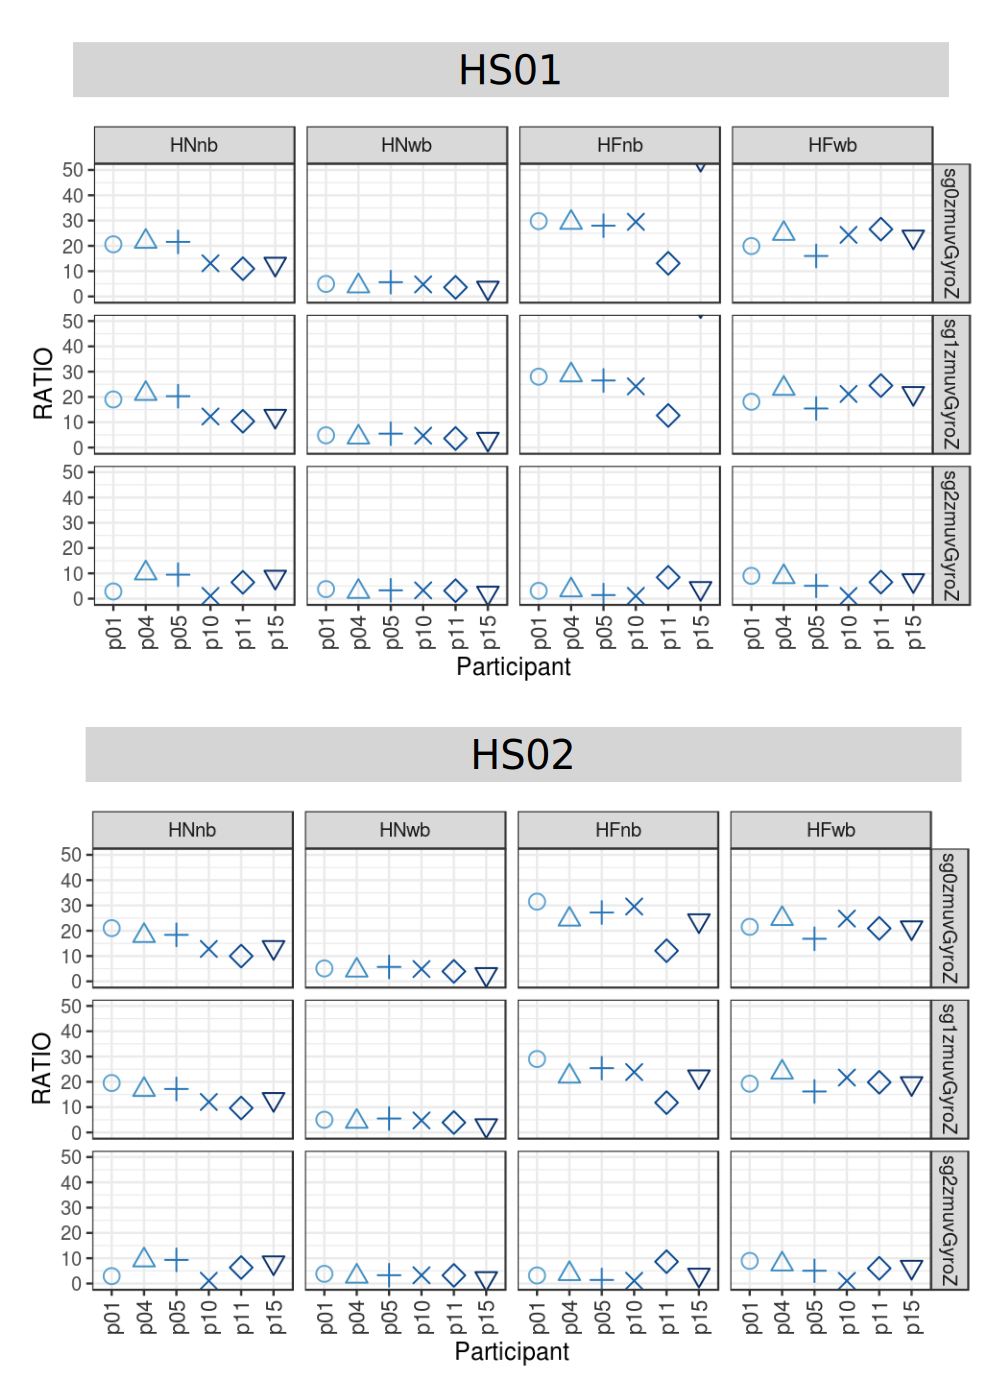
\includegraphics[width=0.9\textwidth]{rqa_ratio_H_w500}
    \caption{
	{\bf RATIO values for horizontal arm movements.}	
	RATIO values, representing dynamic transitions, 
	for 6 participants performing horizontal arm movements 
	(HNnb, HNwb, HFnb, HFwb)
	with sensors HS01, HS02 and three smoothed-normalised axis 
	of GyroZ (sg0zmuvGyroZ, sg1zmuvGyroZ and sg2zmuvGyroZ).
	RATIO values were computed with 
	embedding parameters $m=9$, $\tau=6$ and recurrence threshold
	$\epsilon=1$.
	R code to reproduce the figure is available from \cite{hwum2018}.
        }
    \label{fig:rqa_ratio_H}
\end{figure}
%%---------------------------------(FIGURE)------------------------------------
%%---------------------------------(FIGURE)------------------------------------
\begin{figure}[!h]
\centering
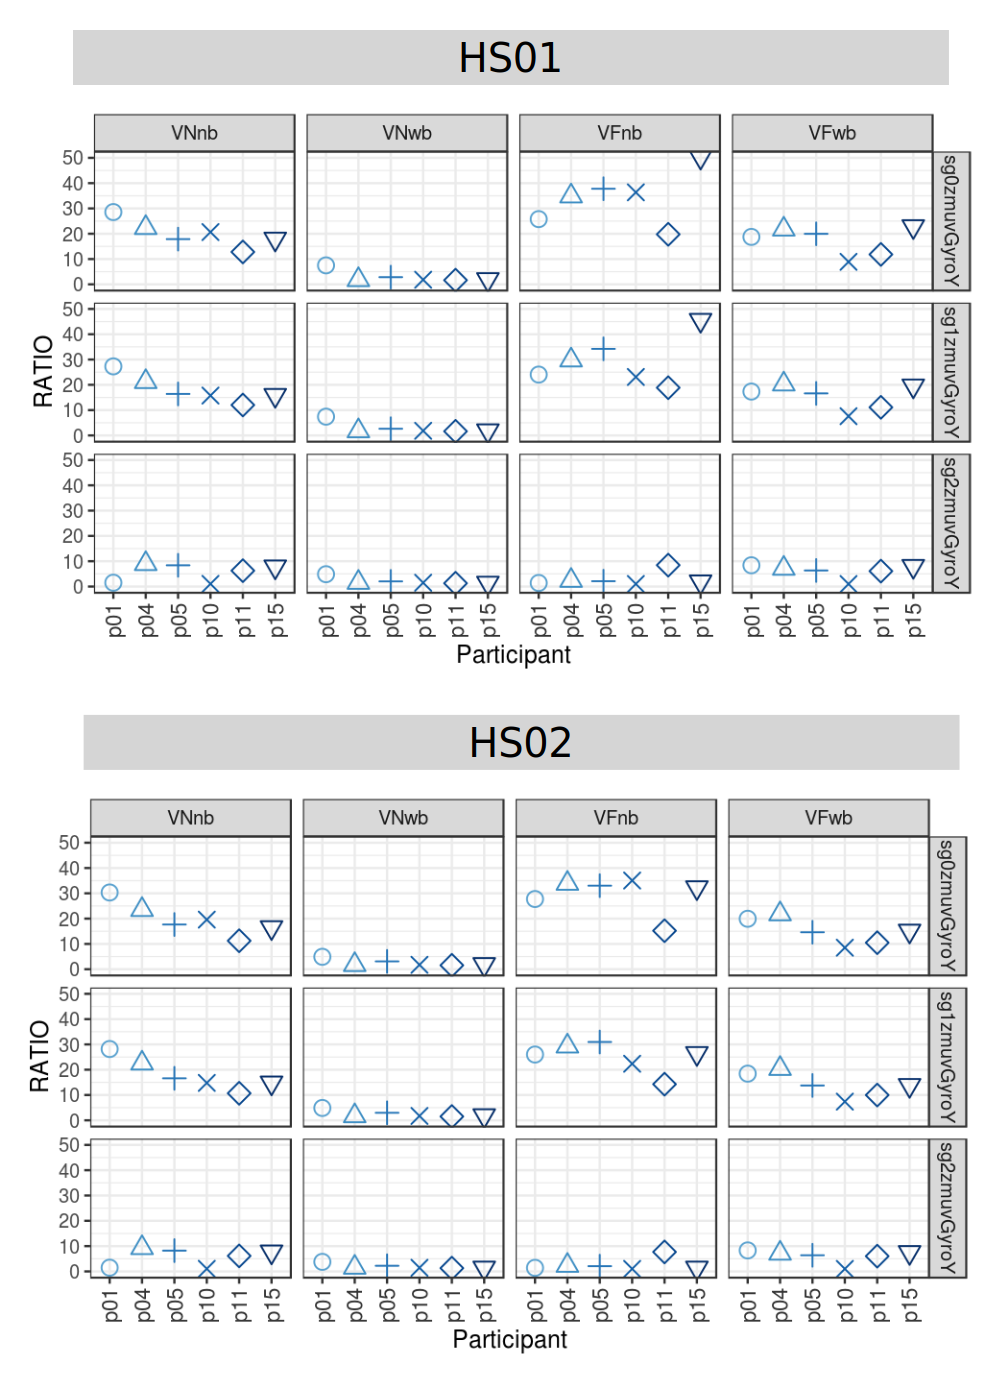
\includegraphics[width=0.9\textwidth]{rqa_ratio_V_w500}
    \caption{
	{\bf RATIO values for vertical arm movements.}	
	RATIO values, representing dynamic transitions, 
	for 6 participants performing vertical arm movements 
	(VNnb, VNwb, VFnb, VFwb)
	with sensors HS01, HS02 and three smoothed-normalised axis 
	of GyroY (sg0zmuvGyroY, sg1zmuvGyroY and sg2zmuvGyroY).
	RATIO values were computed with 
	embedding parameters $m=9$, $\tau=6$ and recurrence threshold
	$\epsilon=1$.
	R code to reproduce the figure is available from \cite{hwum2018}.
        }
    \label{fig:rqa_ratio_V}
\end{figure}
%%---------------------------------(FIGURE)------------------------------------



\subsection{ENTR values}
ENTR values, representing the complexity of the deterministic structure 
of time series, for horizontal and vertical arm movements are shown 
in Figs \ref{fig:rqa_entr_H} and \ref{fig:rqa_entr_V}.

Figs \ref{fig:rqa_entr_H} show ENTR values for horizontal arm movements.
ENTR values appear to be similar for sg0zmuvGyroZ and sg1zmuvGyroZ 
and oscillate between 2 to 4, while ENTR values for sg2zmuvGyroZ appear 
to show similar fluctuations but with higher ENTR values oscillating 
between 3.5 to 5  with the exception of $p10$ with activities VNnb and VFwb 
for sg2zmuvGyroY which ENTR values are slightly out of range.
ENTR values appear to be similar for sensor HS01 and HS02.

Figs \ref{fig:rqa_entr_V} show ENTR values for vertical arm movements.
ENTR values for sg0zmuvGyroY and sg1zmuvGyroY appear to show the same
values and oscillate between 2 to 4, while ENTR values appear to oscillate
between 3.5 to 5 with the exception of $p10$ with activities VNnb and VFwb 
for sg2zmuvGyroY which ENTR values are out of range.
ENTR values for sensor HS01 and HS02 appear to show the same values. 

%%---------------------------------(FIGURE)------------------------------------
\begin{figure}[!h]
\centering
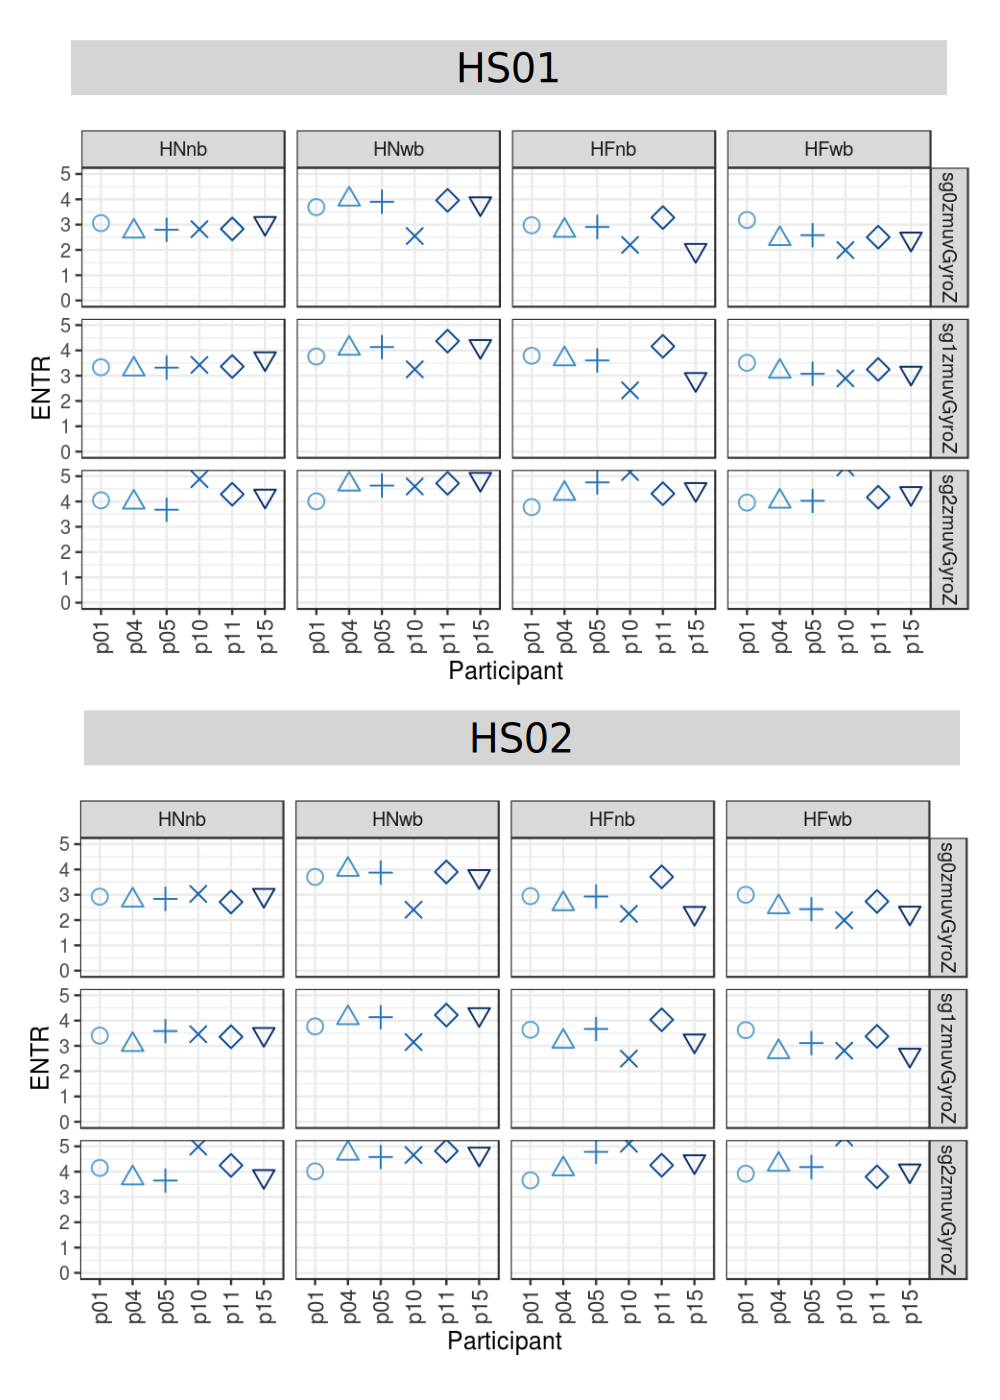
\includegraphics[width=0.88\textwidth]{rqa_entr_H_w500}
    \caption{
	{\bf ENTR values for horizontal arm movements.}
	ENTR values (representing the complexity of the deterministic 
	structure in time series) for 
	6 participants performing horizontal arm movements 
	(HNnb, HNwb, HFnb, HFwb)
	for sensors HS01, HS02 and three smoothed-normalised axis 
	of GyroZ (sg0zmuvGyroZ, sg1zmuvGyroZ and sg2zmuvGyroZ).
	ENTR values were computed with 
	embedding parameters $m=9$, $\tau=6$ and recurrence threshold
	$\epsilon=1$.
	R code to reproduce the figure is available from \cite{hwum2018}.
        }
    \label{fig:rqa_entr_H}
\end{figure}
%%---------------------------------(FIGURE)------------------------------------
%%---------------------------------(FIGURE)------------------------------------
\begin{figure}[!h]
\centering
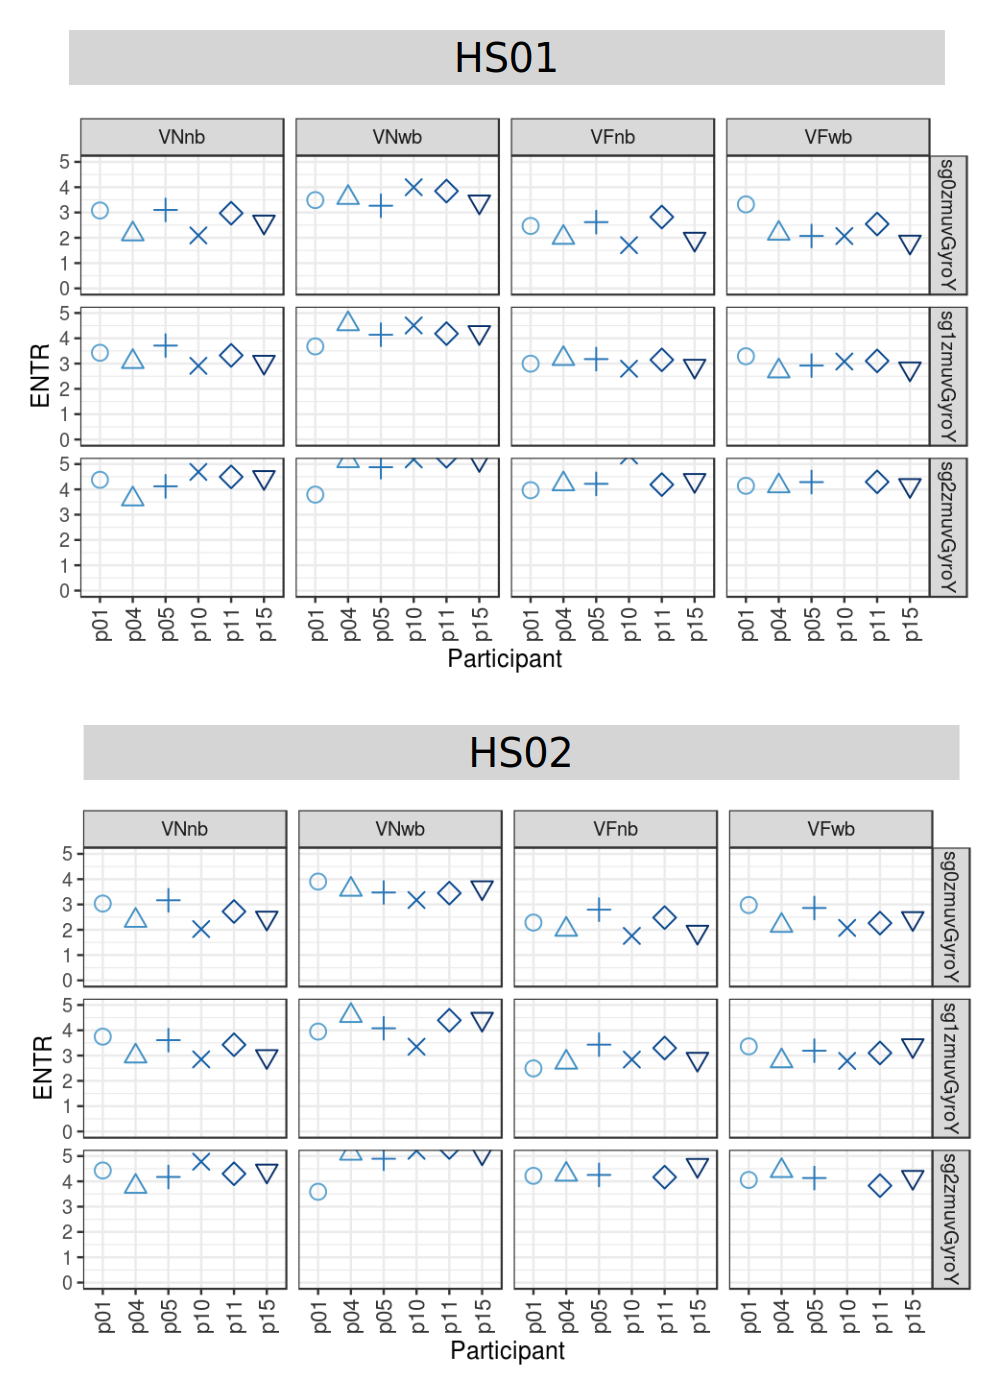
\includegraphics[width=0.88\textwidth]{rqa_entr_V_w500}
    \caption{
	{\bf ENTR values for vertical arm movements.}	
	ENTR values (representing the complexity of the deterministic 
	structure in time series) for 
	6 participants performing vertical arm movements (VNnb, VNwb, VFnb, VFwb)
	for sensors HS01, HS02 and three smoothed-normalised axis 
	of GyroY (sg0zmuvGyroY, sg1zmuvGyroY and sg2zmuvGyroY).
	ENTR values were computed with 
	embedding parameters $m=9$, $\tau=6$ and recurrence threshold
	$\epsilon=1$.
	R code to reproduce the figure is available from \cite{hwum2018}.
        }
    \label{fig:rqa_entr_V}
\end{figure}
%%---------------------------------(FIGURE)------------------------------------



\section{The weaknesses and strengths of RQA}
Surfaces for RQA metrics (REC, DET, RATIO, ENTR) are computed with the 
variation of embedding values by an increase of one 
($0 \ge m \le 10$, $0 \ge \tau \le 10$) 
and recurrence thresholds by an increase of 0.1 ($0.2 \ge \epsilon \le 3$).
Hence, we show different characteristics of 3D surfaces of RQA considering 
different activities, sensors, window size lengths and level of smoothness 
and participants.

Figs \ref{fig:topo_rqas_w500} show the surfaces for RQA metrics 
(REC, DET, RATIO, ENTR) using time series of participant $p01$, 
sensor HS01, activity HNnb, sg0zmuvGyroZ axis and a 500 window 
size length.
The 3D surface for REC values, representing the \% of recurrence dots 
in the RP, show highest values of REC when embedding values 
are near to 1 and the recurrence threshold is at the maximum 
($\epsilon = 3$ for this surfaces). Similarly, it can be seen a decrease
of REC values as the embedding dimension and embedding delay values 
increase, however there is an increase of REC values as the recurrence 
threshold is increasing (Fig \ref{fig:topo_rqas_w500}(A)).
Regarding the 3D surface for DET values, representing predictability 
and organisation of the RPs, Fig \ref{fig:topo_rqas_w500}(B) show slightly 
uniform values when varying both embedding parameters and recurrence 
threshold with the exception of embedding parameters near to 1 and 
recurrence thresholds near to 0.2 where the DET values are smaller.
3D surface for RATIO values, representing dynamic transitions, show 
a plateau with low values recurrence threshold values greater than 1.0.
However, there is a fluctuated increase of RATIO values as the embedding 
values increase given that the recurrence threshold is lower 
than 1 (Fig \ref{fig:topo_rqas_w500}(C)).
For ENTR values, representing the complexity of the structure of the 
time series, Fig \ref{fig:topo_rqas_w500}(D) show a maximum value of 
ENTR when embedding parameters are near to 1 and recurrence threshold values
are near to 3.0. It can also be noted fluctuations in the 3D surface 
when ENTR values are greater than 2.5 (red surface) for embedding 
dimensions between 3 to 9 and a decrease of ENTR values per each 
embedding dimension for delay embedding values (yellow surface).
Additionally, ENTR values decrease as the embedding dimension and 
delay embedding decrease.
%%---------------------------------(FIGURE)-----------------------------------
\begin{figure}[!ht]
\centering
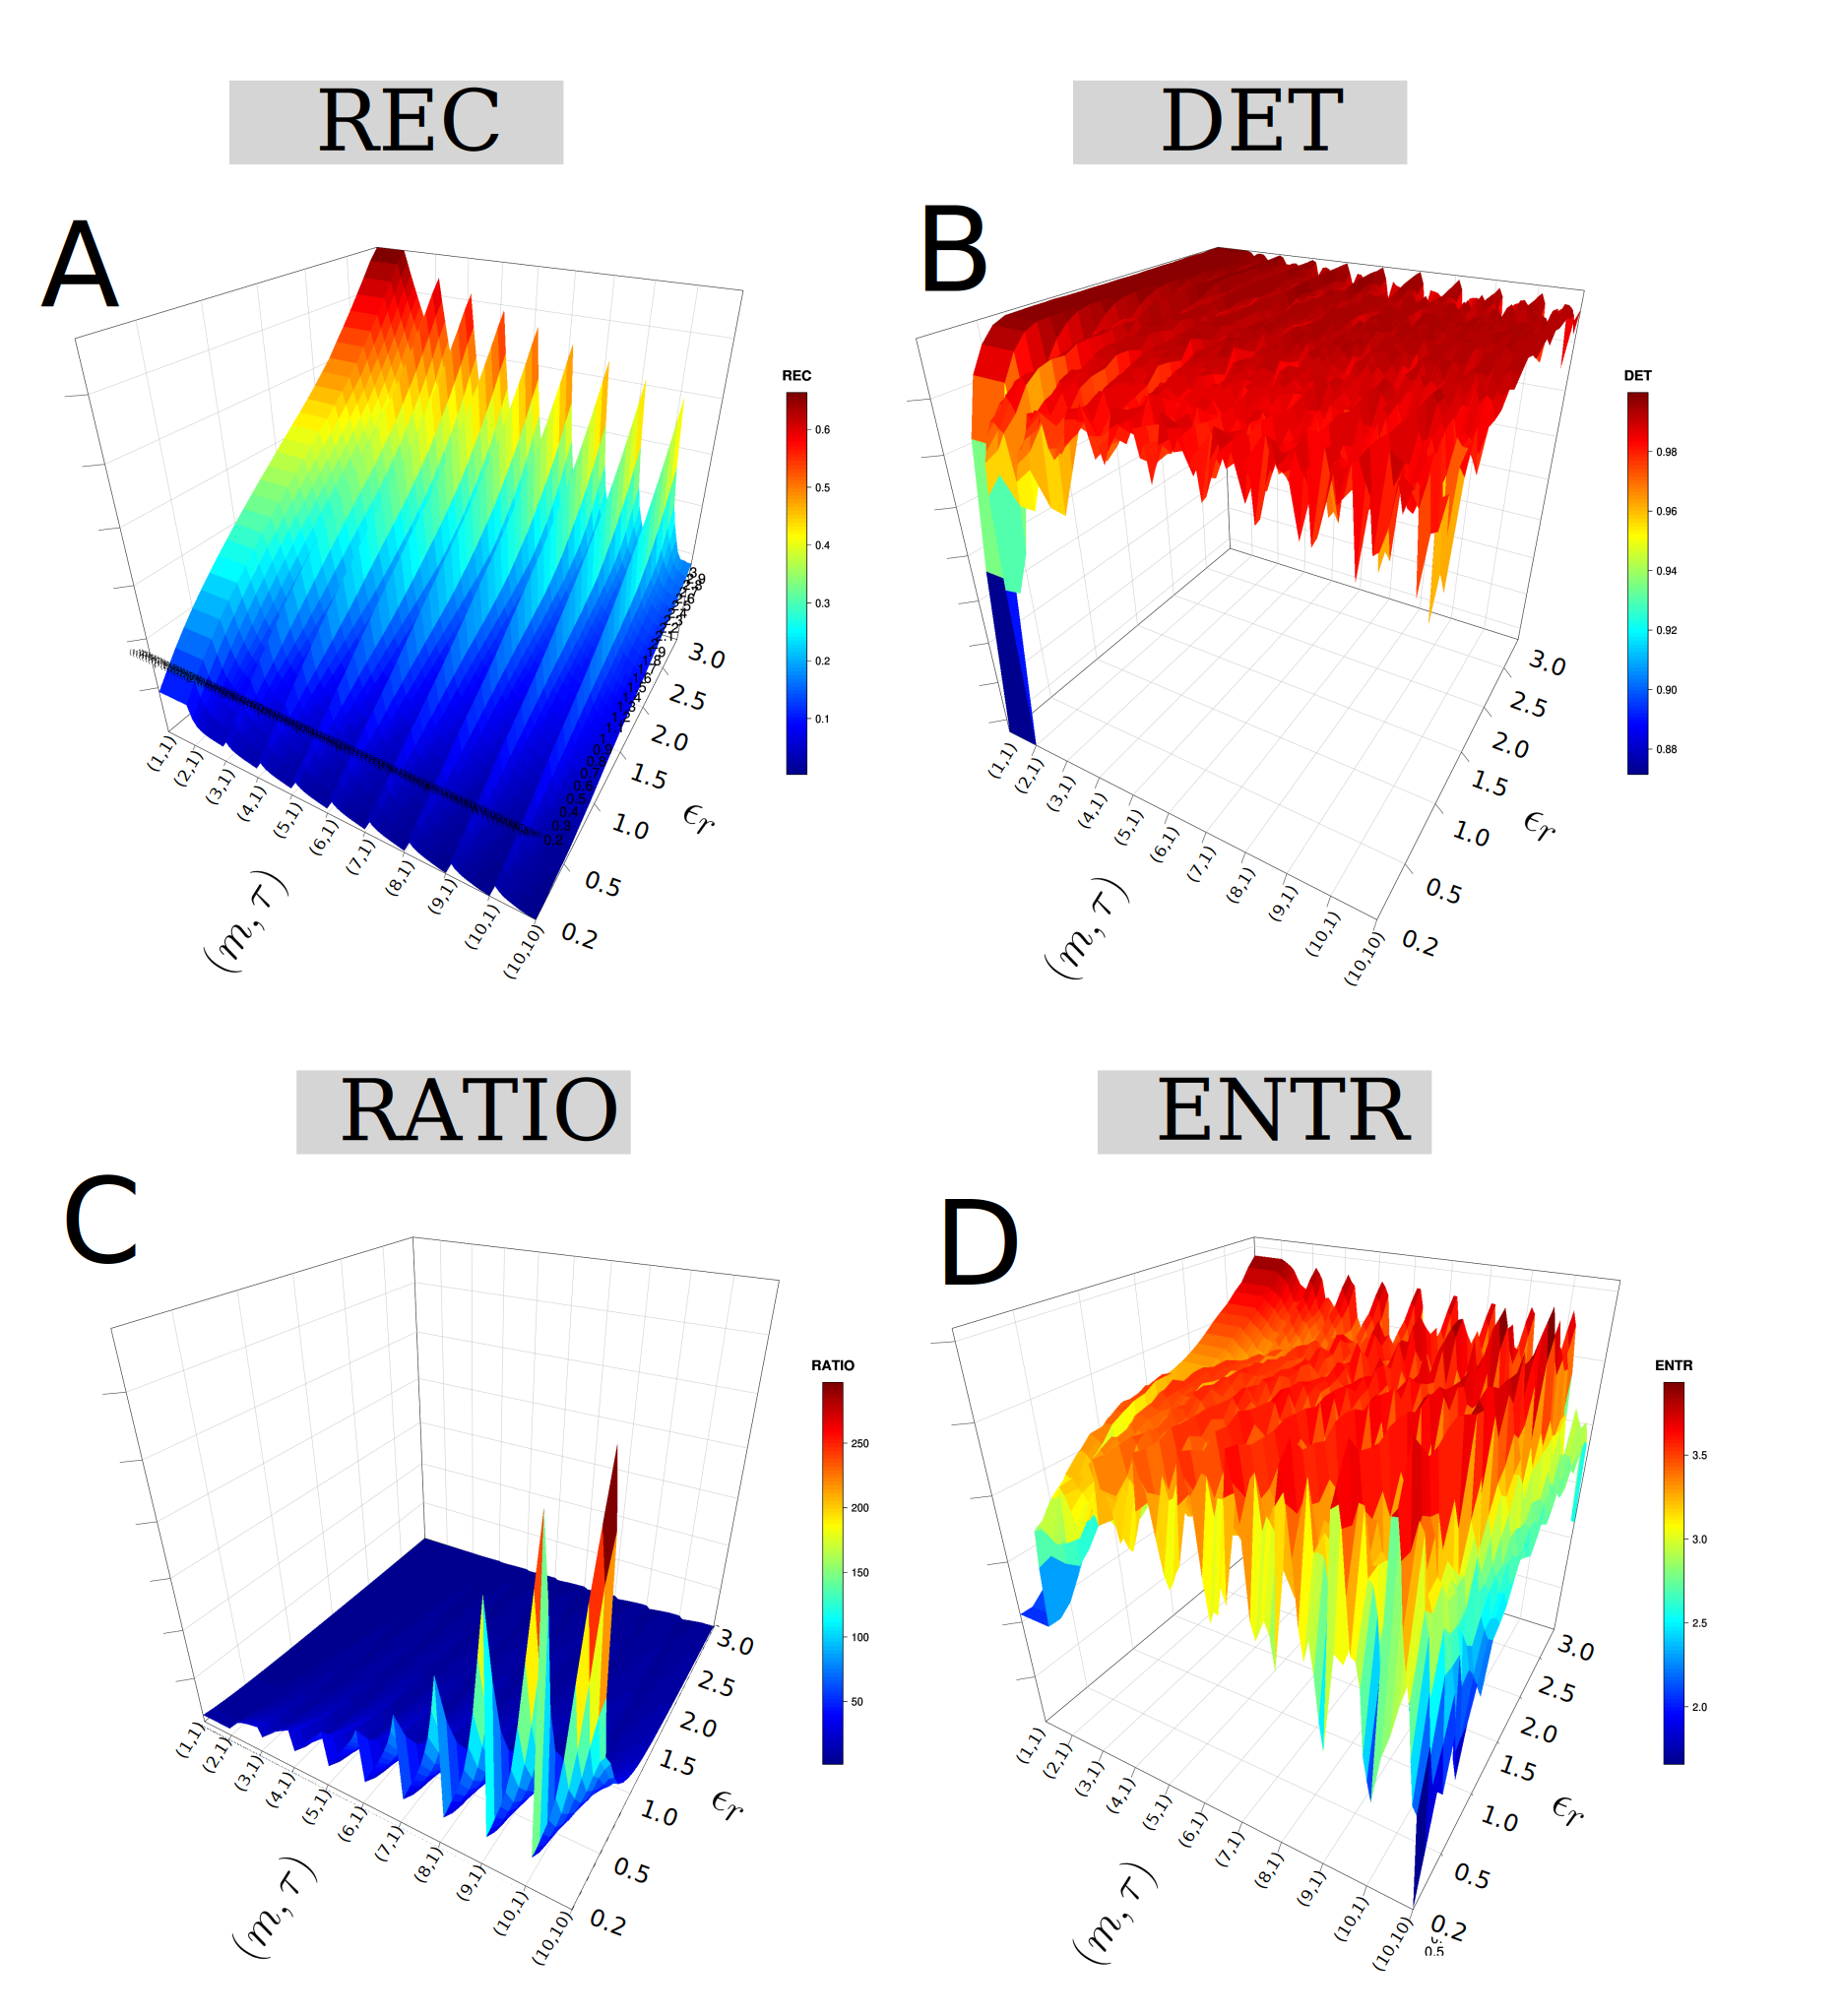
\includegraphics[width=1.0\textwidth]{rqas_w500}
    \caption{
	{\bf 3D surfaces for RQA metrics.}
	3D surfaces for RQA values (A) REC, (B) DET, (C) RATIO and 
	(D) ENTR with an increasing pair of embedding parameters 
	($0 \ge m \le 10$, $0 \ge \tau \le 10$) 
	and recurrence thresholds ($ 0.2 \ge \epsilon \le 3 $).
	RQA metrics are computed with the time series of participant $p01$ using 
	HS01 sensor, HNnb activity, sg0zmuvGyroZ axis and 500 samples 
	for window size length.
        R code to reproduce the figure is available from \cite{hwum2018}.
	}
\label{fig:topo_rqas_w500}
\end{figure}
%%---------------------------------(FIGURE)------------------------------------


\subsection{Sensors and activities}
Figs \ref{fig:topo_s_hs01_H_w500} and \ref{fig:topo_s_hs02_H_w500} show
3D surfaces of RQA metrics (REC, DET, RATIO, ENTR) for horizontal arm 
movements (HNnb, HNwb, HFnb, HFwb) using sensor HS01 and HS02 
for participant $p01$ with sg0zmuvGyroZ axis and 500 window size lenght.
Hence, Figs \ref{fig:topo_s_hs01_H_w500} present 3D surfaces of RQA metrics 
for HS01, where 3D surfaces for REC values 
(Fig \ref{fig:topo_s_hs01_H_w500}(A)) appear to be similar across 
the activities (HNnb, HFnb, HFwb) with the exception of HNwb which 
decrease of REC values is mainly affected by the increase of recurrence 
threshold and slightly affected to the increase of embedding dimension 
parameters. For DET values, 3D surfaces in Figs \ref{fig:topo_s_hs01_H_w500}(B)
appear to show values near to 1.0 (red colour surface), however HNwb 
shown fluctuations of DET values as the embedding dimension increase, 
it can also be noted a decrease of DET values for certain values of 
recurrence threshold (2.6 for HNwb, 0.3 for HFnb, and 0.3 for HFwb).
For Fig \ref{fig:topo_s_hs01_H_w500}(C)), 3D surfaces for RATIO values 
appear to be similar, showing a plateau for values between 0 to 50 
(blue surface) and the increase of peaks is different for each of the 
activities.
For Fig \ref{fig:topo_s_hs01_H_w500}(D), ENTR values present different 
surface formations, for instance, 
HNnb show fluctuated higher values of ENTR (red colour surface),
whereas for activity HNwb the ENTR values are higher (red colour surface) 
for recurrence threshold near to 3.0,
ENTR values for HFnb appear to be higher when embedding dimension is near 
to 10, while higher values for ENTR values for HFwb appear to be 
when the recurrence threshold is near to 0.2.

Then, looking and comparing visually one by one of the surfaces for sensors 
HS01 and HS02 in Figs \ref{fig:topo_s_hs01_H_w500} 
and \ref{fig:topo_s_hs02_H_w500}, one can notice little differences in the 
shape of the surfaces.
Similarly, there is little variations in the surfaces for vertical arm 
movements with the sensors HS01 and HS02 
(Figs \ref{fig:topo_s_hs01_V_w500} and \ref{fig:topo_s_hs02_V_w500}).

With regards to horizontal and vertical movements, 
3D surfaces appear to be similar for REC, DET and RATIO values
with sensor HS01
(Figs \ref{fig:topo_s_hs01_H_w500} and \ref{fig:topo_s_hs01_V_w500})
and sensor HS02
(Figs \ref{fig:topo_s_hs02_H_w500} and \ref{fig:topo_s_hs02_V_w500}), 
however 3D surfaces for ENTR values in each of the arm movements
presents distinguishable variations in the surfaces,
see Figs \ref{fig:topo_s_hs01_H_w500}(D) and \ref{fig:topo_s_hs01_V_w500}(D) 
for horizontal and vertical arm movements with sensor HS01 and
Figs \ref{fig:topo_s_hs02_H_w500}(D) and \ref{fig:topo_s_hs02_V_w500}(D) 
for horizontal and vertical arm movements with sensor HS02.


%%---------------------------------(FIGURE)------------------------------------
\begin{figure}[!ht]
\centering
\includegraphics[width=1.0\textwidth]{s_hs01_H_w500}
    \caption{
	{\bf 3D surfaces of RQA metrics for horizontal arm movements with HS01.}
	3D surfaces for (A) REC, (B) DET, (C) RATIO and (D) ENTR values 
	with increasing pair of embedding parameters 
	($0 \ge m \le 10$, $0 \ge \tau \le 10$) 
	and recurrence thresholds ($ 0.2 \ge \epsilon \le 3 $).
	RQA metrics are computed with the time series of participant $p01$ 
	for sensors HS01, horizontal arm movement activities 
	(HNnb, HNwb, HFnb, HFwb) and 
	sg0zmuvGyroZ axis with 500 samples window size length. 
        R code to reproduce the figure is available from \cite{hwum2018}.
	}
\label{fig:topo_s_hs01_H_w500}
\end{figure}
%%---------------------------------(FIGURE)------------------------------------

%%---------------------------------(FIGURE)------------------------------------
\begin{figure}[!ht]
\centering
\includegraphics[width=1.0\textwidth]{s_hs02_H_w500}
    \caption{
	{\bf 3D surfaces of RQA metrics for horizontal arm movements with HS02.}
	3D surfaces for (A) REC, (B) DET, (C) RATIO and (D) ENTR values 
	with increasing pair of embedding parameters 
	($0 \ge m \le 10$, $0 \ge \tau \le 10$) 
	and recurrence thresholds ($ 0.2 \ge \epsilon \le 3 $).
	RQA metrics are computed with the time series of participant $p01$ 
	for sensors HS02, horizontal arm movement activities 
	(HNnb, HNwb, HFnb, HFwb) and 
	sg0zmuvGyroZ axis with 500 samples window size length. 
        R code to reproduce the figure is available from \cite{hwum2018}.
	}
\label{fig:topo_s_hs02_H_w500}
\end{figure}
%%---------------------------------(FIGURE)------------------------------------

%%---------------------------------(FIGURE)-----------------------------------
\begin{figure}[!ht]
\centering
\includegraphics[width=1.0\textwidth]{s_hs01_V_w500}
    \caption{
	{\bf 3D surfaces of RQA metrics for vertical arm movements with HS01.}
	3D surfaces for (A) REC, (B) DET, (C) RATIO and (D) ENTR values 
	with increasing pair of embedding parameters 
	($0 \ge m \le 10$, $0 \ge \tau \le 10$) 
	and recurrence thresholds ($ 0.2 \ge \epsilon \le 3 $).
	RQA metrics are computed with the time series of participant $p01$ 
	for sensors HS01, vertical arm movements activities 
	(VNnb, VNwb, VFnb, VFwb) and 
	sg0zmuvGyroY axis with 500 samples window size length. 
        R code to reproduce the figure is available from \cite{hwum2018}.
	}
\label{fig:topo_s_hs01_V_w500}
\end{figure}
%%---------------------------------(FIGURE)------------------------------------


%%---------------------------------(FIGURE)------------------------------------
\begin{figure}[!ht]
\centering
\includegraphics[width=1.0\textwidth]{s_hs02_V_w500}
    \caption{
	{\bf 3D surfaces of RQA metrics for vertical arm movements with HS02.}
	3D surfaces for (A) REC, (B) DET, (C) RATIO and (D) ENTR values 
	with increasing pair of embedding parameters 
	($0 \ge m \le 10$, $0 \ge \tau \le 10$) 
	and recurrence thresholds ($ 0.2 \ge \epsilon \le 3 $).
	RQA metrics are computed with the time series of participant $p01$ 
	for sensors HS02, vertical arm movements activities 
	(VNnb, VNwb, VFnb, VFwb) and 
	sg0zmuvGyroY axis with 500 samples window size length. 
        R code to reproduce the figure is available from \cite{hwum2018}.
	}
\label{fig:topo_s_hs02_V_w500}
\end{figure}
%%---------------------------------(FIGURE)------------------------------------


\subsection{Window size}
3D surfaces of REC values with a short window length (100 samples) can affect
the shape of 3D surface, however for window size of 250, 500, and 700 samples,
the 3D surfaces appear to show little changes 
(Figs \ref{fig:topo_windows_hii}(A)).
For instance, one can see 3D surfaces of DET values with a window of 100 
size length is slightly different to other surfaces but keeping the plateau
(red surface) in each of the surfaces (Figs \ref{fig:topo_windows_hii}(B)).
Similarly, the 3D surfaces of RATIO values preserve the same plateau 
(blue surface) with little variations in the surfaces as window size length 
increase (Figs \ref{fig:topo_windows_hii}(C)).
3D surfaces for ENTR values appear to have similar aspects as the 
fluctuations of the curves keeps the same values (red and yellow colours).
It can also be noted that the smoothness of 3D surfaces decrease as the 
embedding dimension parameters increase and such smoothness is also affected 
by the window length (see Figs \ref{fig:topo_windows_hii}(D)).


%---------------------------------(FIGURE)-------------------------------------
\begin{figure}[!ht]
\centering
\includegraphics[width=1.0\textwidth]{windowlength}
    \caption{
	{\bf 3D surfaces of RQAs metrics for different window size lengths.}
	3D surfaces of RQA metrics ((A) REC, (B) DET, (C) RATIO, and (D) ENTR) 
	with increasing embedding 
	parameters and recurrence thresholds for four window 
	lengths (w100, w250, w500 and  w750).
	RQA metrics values are for time series of participant p01 
	using HS01 sensor, HNnb activity and sg0zmuvGyroZ axis.
	R code to reproduce the figure is available from \cite{hwum2018}.
       }
\label{fig:topo_windows_hii}
\end{figure}
%%---------------------------------(FIGURE)------------------------------------


\subsection{Smoothness}
Figs \ref{fig:topo_smoothness_hii} show the effects of three levels of 
smothness (sg0zmuvGyroZ, sg1zmuvGyroZ and sg2zmuvGyroZ) in the RQA metrics.
Generally, 3D surfaces from sg2zmuvGyroZ are affected by the smoothness.
It can also be noted that REC values and ENTR values present a slightly 
different surfaces (see Figs \ref{fig:topo_smoothness_hii}(A, D)), 
while DET and RATIO values appear to be similar which is mainly reflected in 
the colour of the curves (see Figs \ref{fig:topo_smoothness_hii}(B, C)).
In Figs \ref{fig:topo_smoothness_hii}(A), 3D surfaces for REC values tend be 
smoothed as the smoothness of the time series increase to the point where 
the increase of recurrence threshold affects the shape of the surfaces.
Similarly, in Figs  \ref{fig:topo_smoothness_hii}(C), 
3D surface for ENTR values is affected by the smoothness of the 
time series to the point that the fluctuations in the surface does change 
drastically the shape by showing only an increase of ENTR values as
the recurrence threshold increase.

%%---------------------------------(FIGURE)------------------------------------
\begin{figure}[!ht]
\centering
\includegraphics[width=1.0\textwidth]{smoothness_w500}
    \caption{
	{\bf 3D surfaces of RQA metrics with three levels of smoothness.}
	3D surfaces of RQA metrics ((A) REC, (B) DET, (C) RATIO, and (D) ENTR) 
	with increasing embedding parameters and recurrence thresholds for 
	three levels of smoothness 
	(sg0zmuvGyroZ, sg1zmuvGyroZ, and sg2zmuvGyroZ).
	RQA metrics are computed from time series of participant $p01$ using 
	HS01 sensor, HNnb activity and 500 samples window length.
	R code to reproduce the figure is available from \cite{hwum2018}.
 }
\label{fig:topo_smoothness_hii}
\end{figure}
%%---------------------------------(FIGURE)------------------------------------


\subsection{Participants}
The shape of 3D surfaces of RQA metrics is also affected when using 
time series from different participants (Figs \ref{fig:topo_participants_hii}).
For instance, 3D surface of DET values show slightly but noticeable 
differences in the fluctuations when embedding dimension and recurrence 
threshold increase (Figs \ref{fig:topo_participants_hii}(B)) which is similar 
for ENTR values where the fluctuations of the 3D surfaces changes for each 
of the participants (Figs \ref{fig:topo_participants_hii}(D)).
However, the shape of 3D surfaces for RET values and RATIO values 
is little affected with the change of participants 
(Figs \ref{fig:topo_participants_hii}(A, C)).

%%---------------------------------(FIGURE)------------------------------------
\begin{figure}[!ht]
\centering
\includegraphics[width=1.0\textwidth]{participants_w500}
    \caption{
	{\bf 3D surfaces of RQA metrics with three participants.}
	3D surfaces of RQA metrics ((A) REC, (B) DET, (C) RATIO, and (D) ENTR) 
	for participants $p01$, $p04$ and $p05$ with increasing embedding 
	parameters and recurrence thresholds.
	RQA metrics values are for time series of HS01 sensor, 
	HNnb activity and 500 samples window length.
	R code to reproduce the figure is available from \cite{hwum2018}.
 }
\label{fig:topo_participants_hii}
\end{figure}
%%---------------------------------(FIGURE)-------------------------------------



\subsection{Final remarks}
%	You need to say whether the results are expected and
%	whether different methods agree or contradict each other. \\
Independently of the source of time series, surfaces for RATIO 
values are affected little by the changes of embedding values and recurrence 
thresholds with the exception for the peaks presented when embedding values 
increase for recurrence thresholds less than one. 
Then, 3D surfaces for DET values are affected slightly more than RATIO values
and the changes are also independent of the source of time series.
Nonetheless, REC values are affected by the window size, type of activity 
and level of smoothness.
For ENTR values, we can see that 3D surfaces show clearly differences with 
regards to any of the sources of the time series,
hence making ENTR metric a robust metric to quantify human movement 
variability from different time series.



